\section{Music notation anatomy}

\subsection{Note names}

You have already seen the music staff from \autoref{fig:ukulele_music_note_names_on_staff} in the previous exercises. However, the meaning of it was not explained yet.

The letters A-G on the staff show which line on the staff has which note value. The notes that are in between the lines nicely spell out "\textbf{FACE}", making it easy to remember. The Note that are on the lines can be remembered with the mnemonic "\textbf{E}very \textbf{G}ood \textbf{B}oy \textbf{D}oes \textbf{F}ine". But another important thing to see is that the notes go up alphabetically (starting again with A after G). 

The most left symbol (\clefG) is called the G clef. Note that the inner/middle curl of the G clef is on the line of the G note. 

The vertical line in the middle of the staff indicates the start/end of a measure. and the thicker vertical line at the end indicates the end of the piece.

\begin{figure}[h]
	\centering
	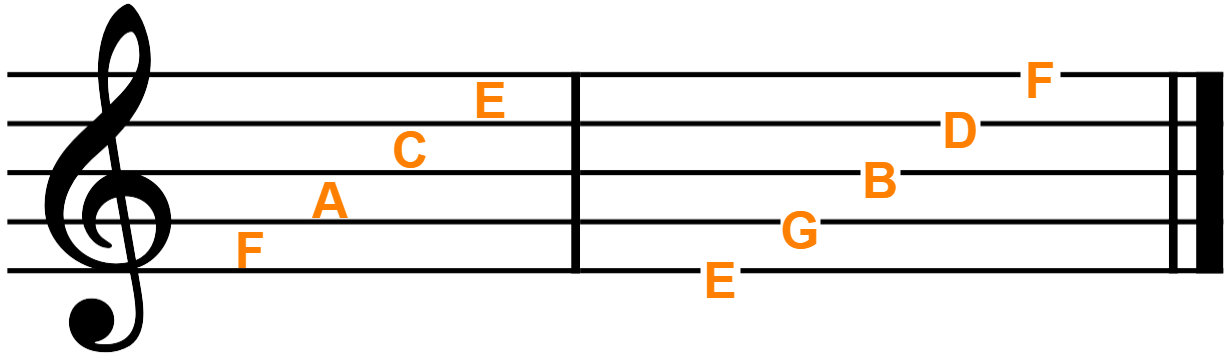
\includegraphics[width=0.6\textwidth]{../../Images/MusicNotation_MeasureNoteNames.png}
	\caption{Note names on the staff in two measures}
	\label{fig:ukulele_music_note_names_on_staff}
\end{figure}

The ukulele is mostly knows for it's happy strumming of chords of course. A chord is a collection of notes. So while it maybe is more fun in the short term to start with strumming chords, is pays off in the the long term to learn your notes and where they are on the fretboard. That way you can be more creative with your chords.

Additionally, training your finger-style playing from the start will help to play melody lines through the chords more easily.

Once we know our notes on the fretboard, we will start to play chords and learn how to construct them from scratch.

\newpage

\subsection{Counting}

So far we have also only seen one type of note. The quarter note. However, there are more. See \autoref{fig:ukulele_note_duration_basic}. The \lilyTimeSignature{4}{4} time signature means that there can fit 4 (top number) quarter notes (bottom number) in a measure. 

\begin{figure}[h]
	\centering
	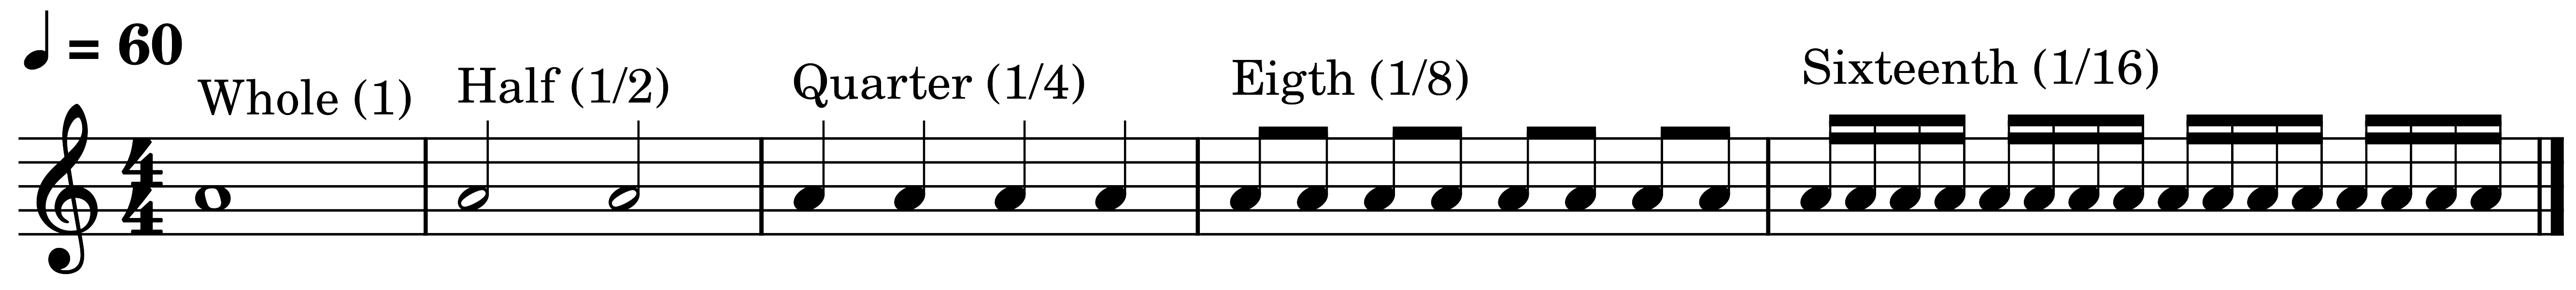
\includegraphics[width=\textwidth]{../../MuseScore/Ukulele/MusicNotation/NoteDurations_Basic.png}
	\caption{Note duration}
	\label{fig:ukulele_note_duration_basic}
\end{figure}

\textbf{Important}: A whole note (\wholeNote) equal 4 quarter notes (\quarterNote). It does \textbf{not} equal a whole measure. \newline

There are also other time signatures. The top value indicates how many notes of the bottom number's duration fit in a measure. So a \lilyTimeSignature{3}{4} time signature can fit 3 quarter notes per measure. And a \lilyTimeSignature{6}{8} time signature can fit 6 eighth notes per measure. Note that \lilyTimeSignature{3}{4} and \lilyTimeSignature{6}{8} indicate the same duration per measure, but they give a different feel. This is demonstrated in \autoref{fig:ukulele_time_signatures}.

In \autoref{fig:ukulele_time_signatures} you also see a new duration notation. In the first measure with \lilyTimeSignature{6}{8} timing, there are dots next to the notes (\quarterNoteDottedDown). This means that the note has a duration of 1.5x its original duration.

The ">" symbol means that this note should be played with a more powerful accent. The \textbf{bold} numbers above the notes indicate the counting of the notes. A bold number means to put an accent on it, but played less accented than the ones where there is also an ">" symbol.

\begin{figure}[h]
	\centering
	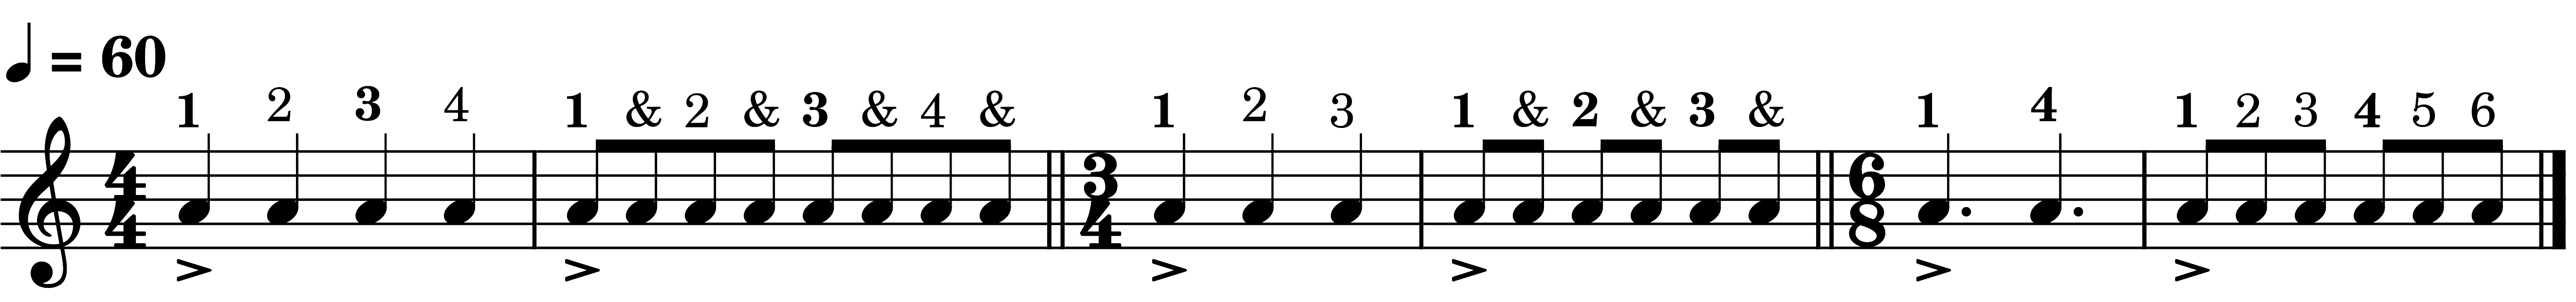
\includegraphics[width=\textwidth]{../../MuseScore/Ukulele/MusicNotation/TimeSignature.png}
	\caption{Time signatures}
	\label{fig:ukulele_time_signatures}
\end{figure}

\newpage

Where notes indicate when to play a sound, rests indicate when to be silent. In \autoref{fig:ukulele_rests} the most common rest durations are shown.

\begin{figure}[h]
	\centering
	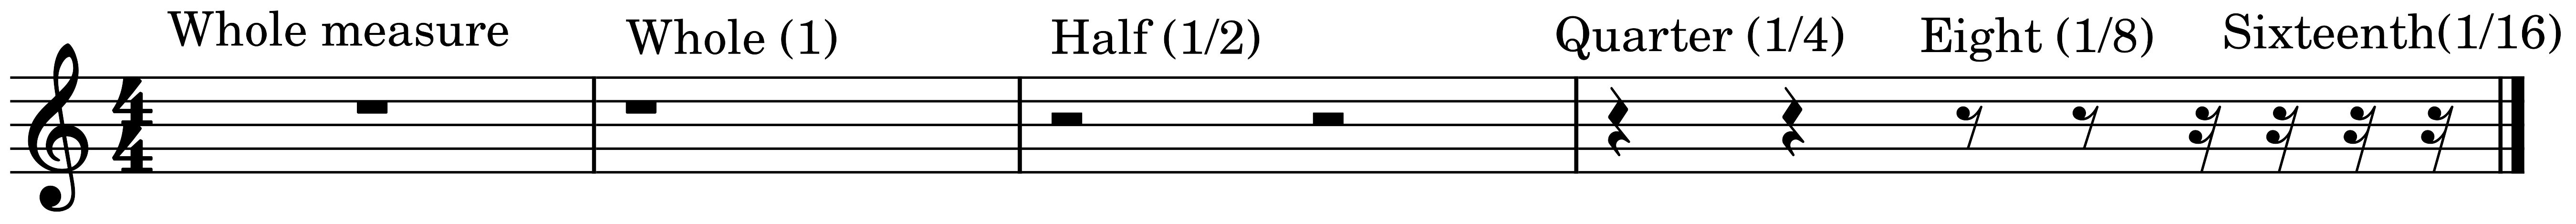
\includegraphics[width=\textwidth]{../../MuseScore/Ukulele/UkuleleRests.png}
	\caption{Rest notations of different duration}
	\label{fig:ukulele_rests}
\end{figure}

In \autoref{fig:ukulele_rests_exercise} an exercise is provide to count the rests. Remember to take this slow and to be conscious about the counts. As a help the tempo is set to the 60 quarter notes per minutes (BPM). This way each quarter note is 1 second. But feel free to play it slower.

It can also be helpful to use a metronome.

\begin{figure}[h]
	\centering
	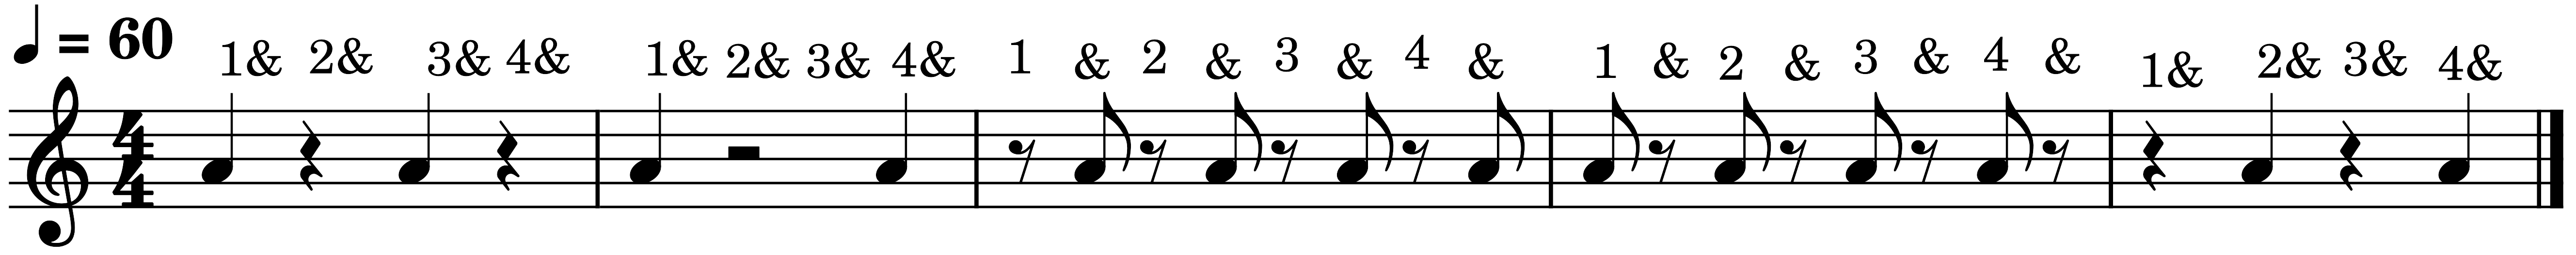
\includegraphics[width=\textwidth]{../../MuseScore/Ukulele/UkuleleRestsExercise.png}
	\caption{Rest notations of different duration}
	\label{fig:ukulele_rests_exercise}
\end{figure}

\newpage

\subsection{Learning the main notes}

To learn the notes we will first start with the well known "Jingle bells". This song uses all non-sharp/flat notes on the 3rd and 2nd string of the ukulele up to the 3rd frets. See \autoref{fig:ukulele_notes_for_jingle_bells} for the tabs of these notes.

Above the notes you see the left-hand fingers to be used. Use alternating \textit{i} and \textbf{m} fingers.

\begin{figure}[h]
	\centering
	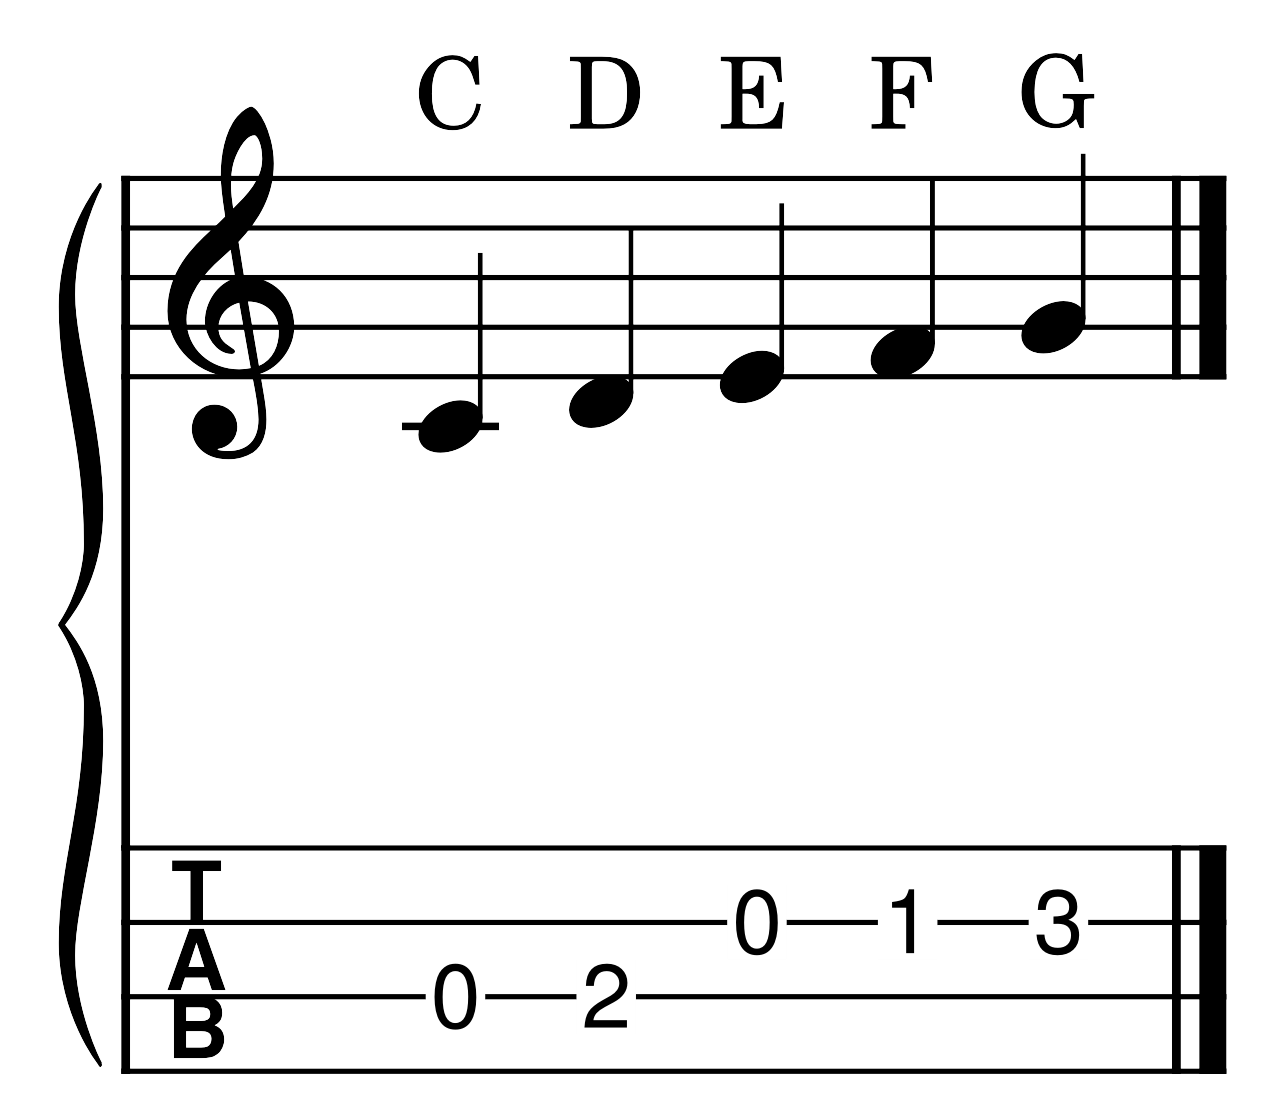
\includegraphics[height=0.12\textheight]{../../MuseScore/Ukulele/UkuleleNotesInJingleBells.png}
	\caption{Notes used for Jingle bells}
	\label{fig:ukulele_notes_for_jingle_bells}
\end{figure}

\begin{figure}[h]
	\centering
	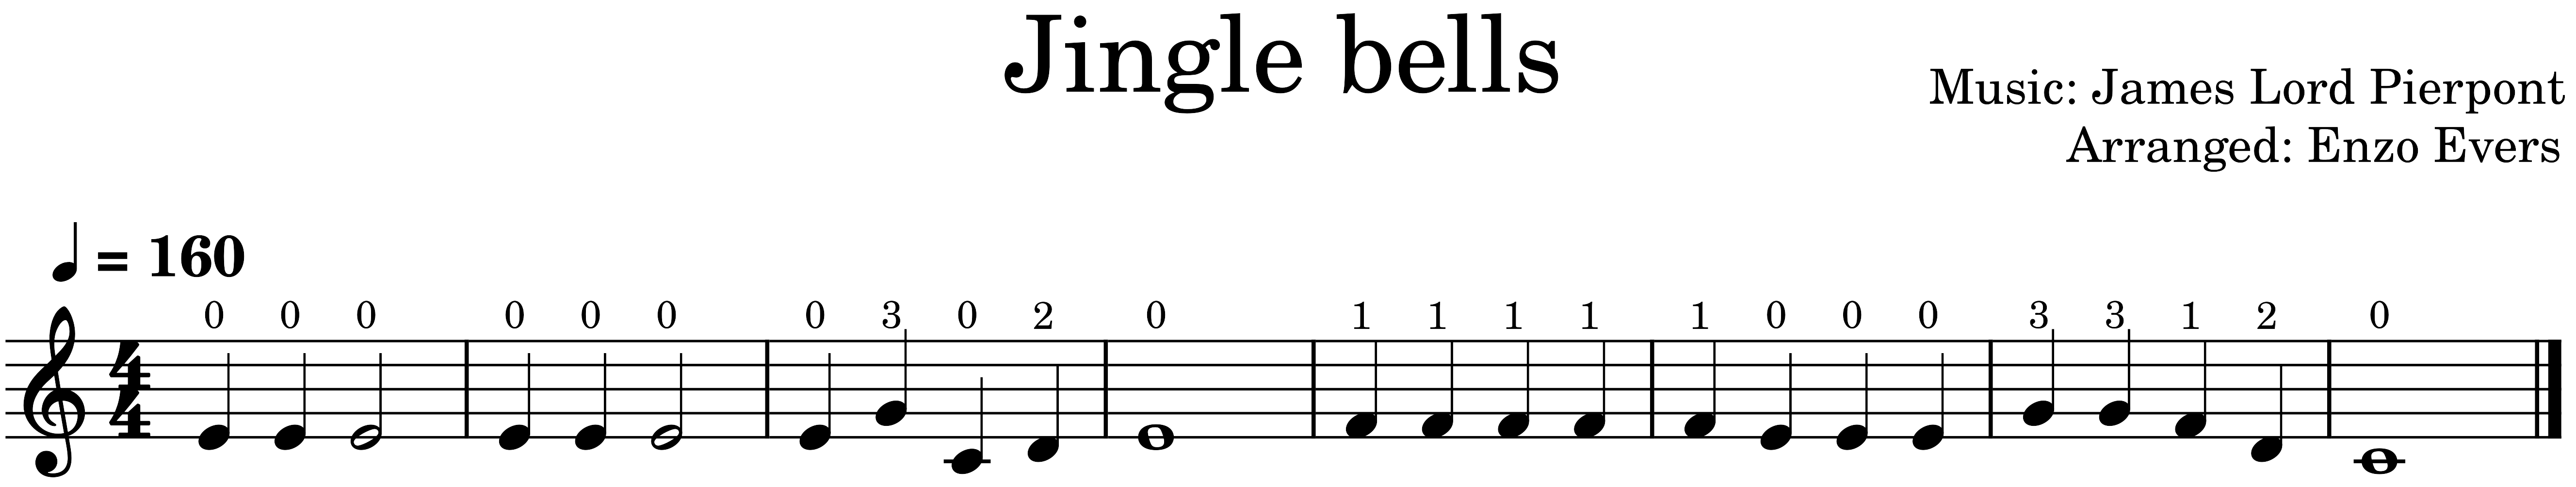
\includegraphics[width=\textwidth]{../../MuseScore/Ukulele/UkuleleJingleBells.png}
	\caption{Jingle bells}
	\label{fig:ukulele_jingle_bells}
\end{figure}

\newpage

In preparation to play the "Tetris" tune, the notes from \autoref{fig:ukulele_notes_for_tetris_first_part} should be learned. Note that only the A note is new compared to the notes in Jingle Bells (\autoref{fig:ukulele_notes_for_jingle_bells}).

\begin{figure}[h]
	\centering
	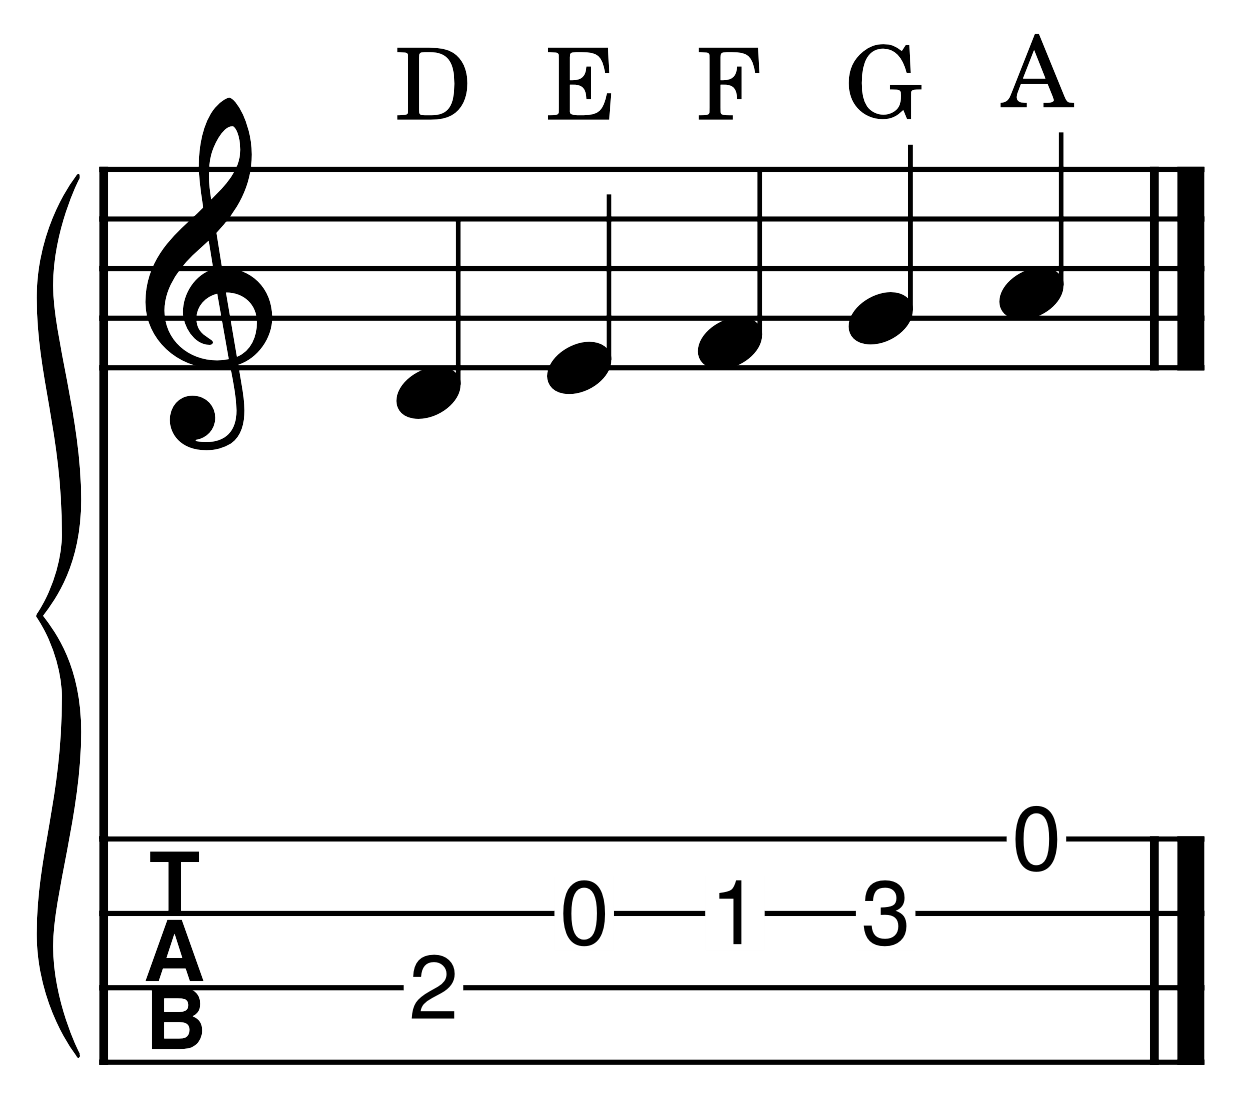
\includegraphics[height=0.12\textheight]{../../MuseScore/Ukulele/UkuleleNotesUsedInTetrisFirstPart.png}
	\caption{Notes used for the first part of the Tetris tune}
	\label{fig:ukulele_notes_for_tetris_first_part}
\end{figure}

\begin{figure}[h]
	\centering
	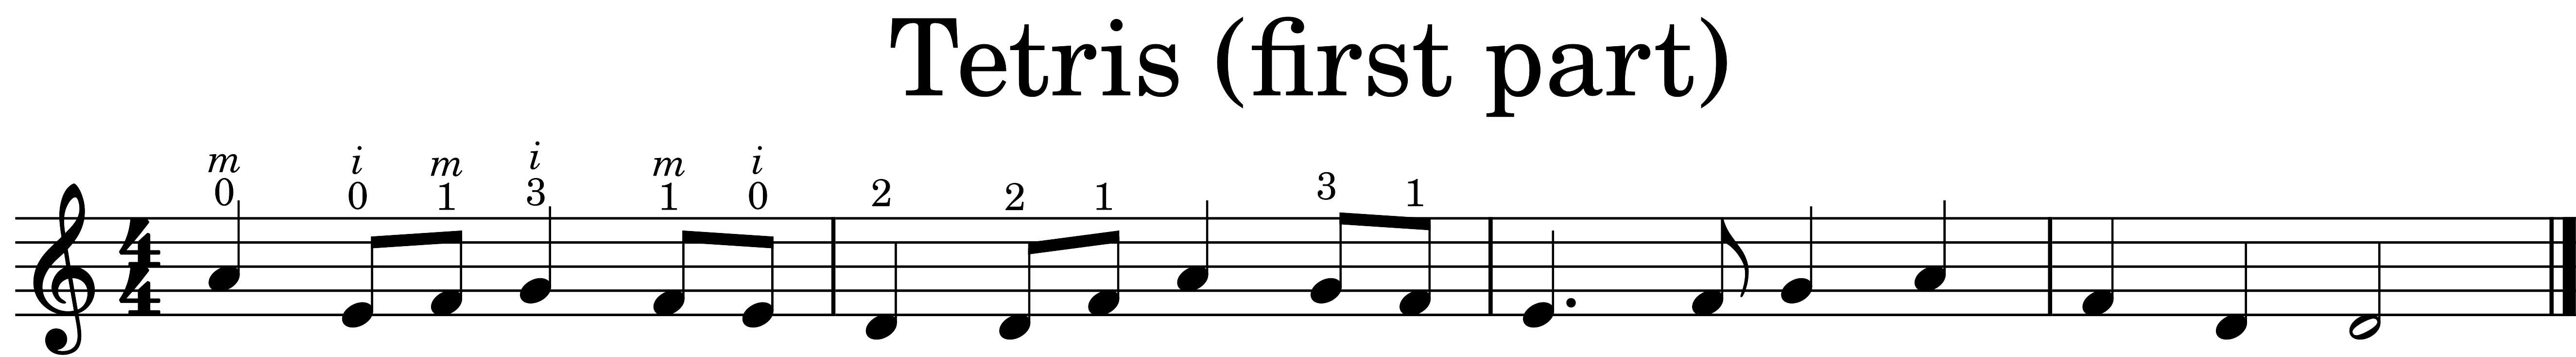
\includegraphics[width=\textwidth]{../../MuseScore/Ukulele/UkuleleTetrisSimpleFirstPart.png}
	\caption{First part of the Tetris tune}
	\label{fig:ukulele_tetris_simple_first_part}
\end{figure}


\infobox{The "Tetris" tune is derived from a Russian folk song called "Korobeiniki", which is based the a similar named poem written by Nikolay Nekrasov. \cite{KorobeinikiWiki}}

\newpage

In the next song you will learn the remaining non-sharp/flat notes on the first string. The B and the C.

\begin{figure}[h]
	\centering
	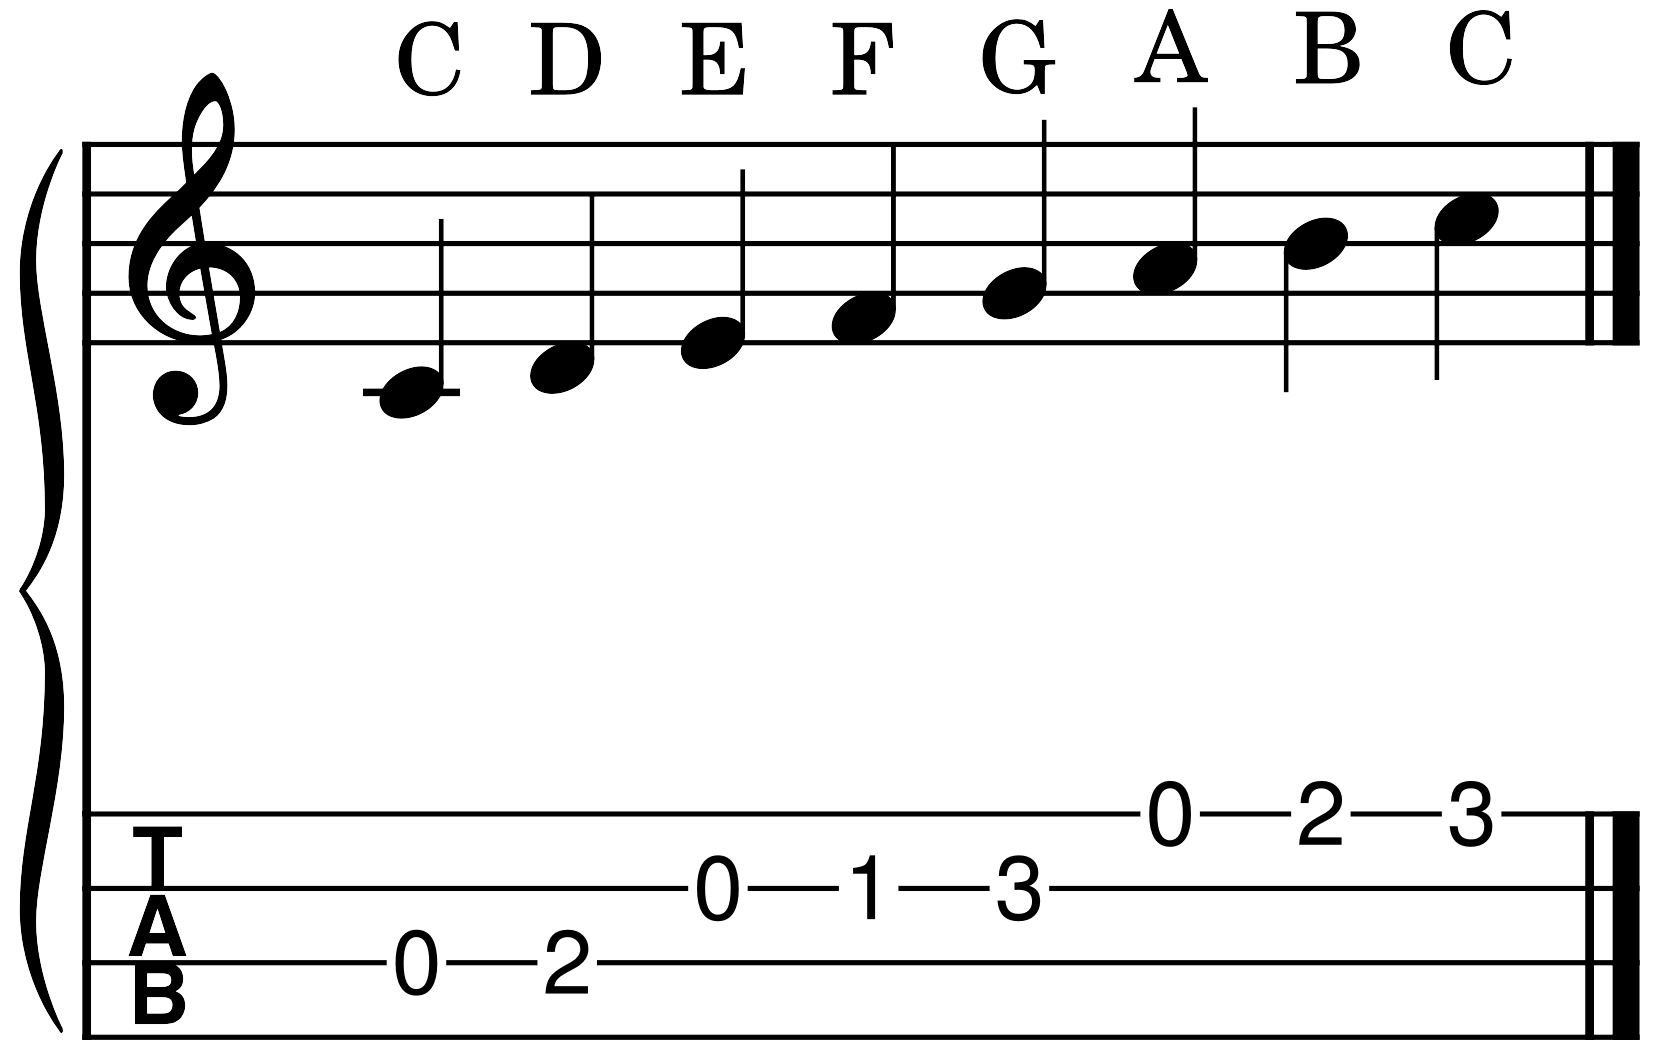
\includegraphics[height=0.12\textheight]{../../MuseScore/Ukulele/UkuleleNotesUsedInVogeltjesdans.png}
	\caption{Notes used for the song "De Vogeltjesdans"}
	\label{fig:ukulele_notes_for_vogeltjesdans}
\end{figure}

\infobox{In \autoref{fig:ukulele_notes_for_vogeltjesdans} you not only see the notes used in the song, but you also see the C major scale. Later on we will talk more about scales.}

\begin{figure}[h]
	\centering
	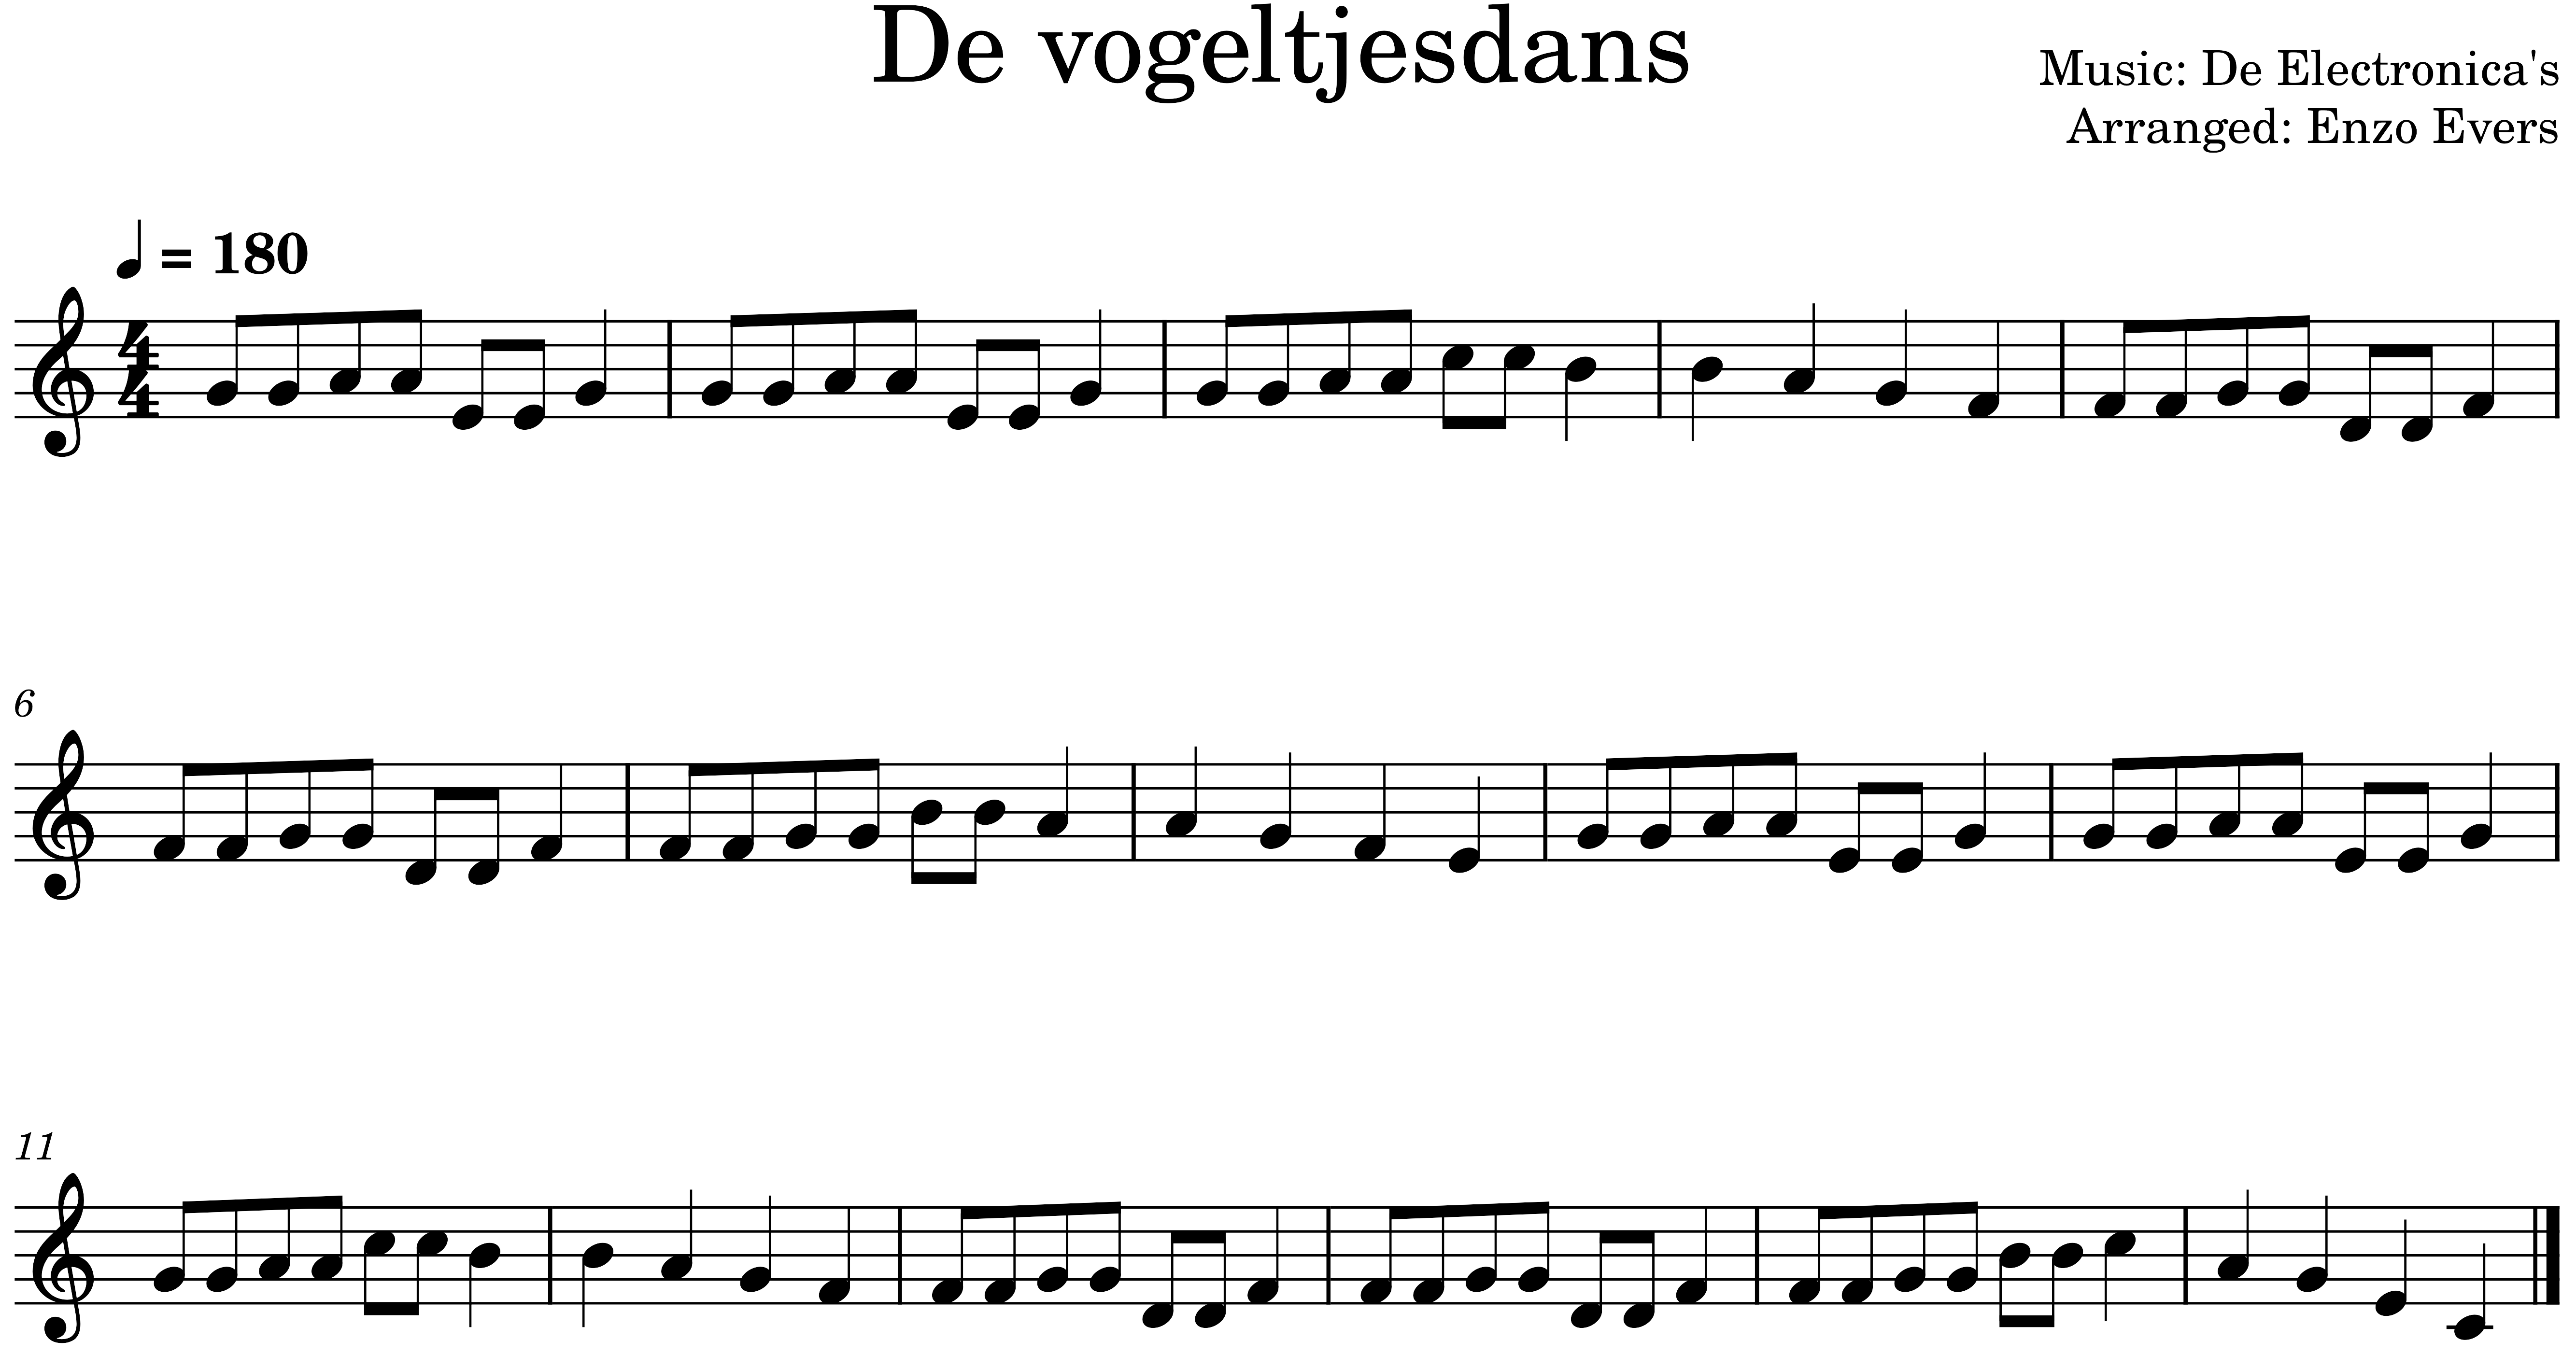
\includegraphics[width=\textwidth]{../../MuseScore/Ukulele/UkuleleVogeltjesdansDeElectronicas.png}
	\caption{De vogeltjesdans - De Electronica's}
	\label{fig:ukulele_vogeltjesdans}
\end{figure}

\infobox{While most people know this as the Dutch titled "De vogeltjesdans", it is based on the original song called "Der Ententanz" composed by Werner Thomas. \cite{DeVogeltjesDansWiki}}

\newpage

No new notes to learn for "Seven Nation Army" (\autoref{fig:ukulele_seven_nation_army}). Note, because of the limited low notes on the ukulele, \autoref{fig:ukulele_seven_nation_army} is played slightly higher compared to the original recording.

\begin{figure}[h]
	\centering
	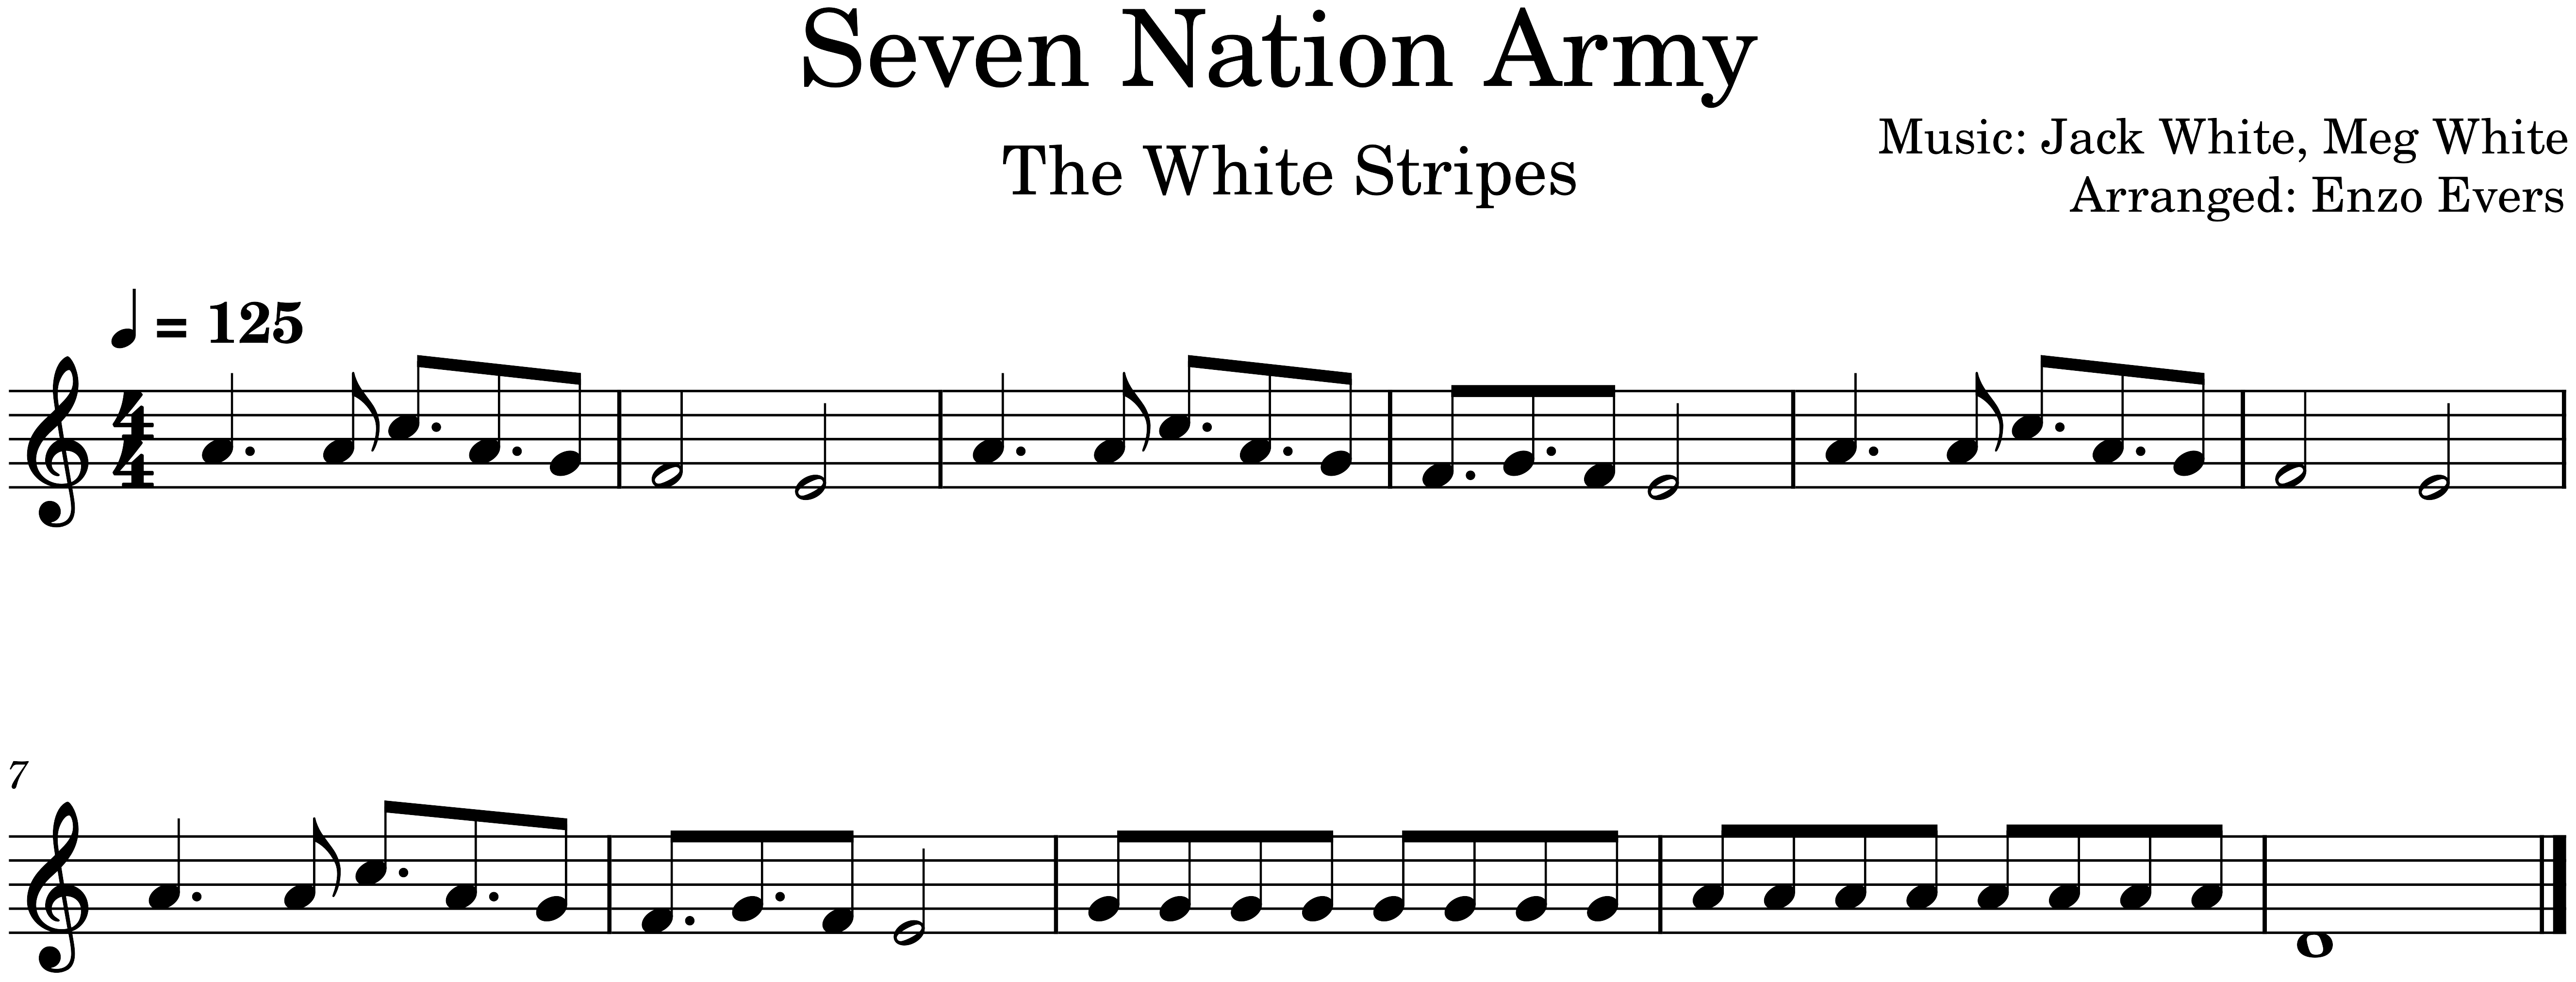
\includegraphics[width=\textwidth]{../../MuseScore/Ukulele/Ukulele_SevenNationArmy-TheWhiteStripes.png}
	\caption{Seven Nation Army - The White Stripes}
	\label{fig:ukulele_seven_nation_army}
\end{figure}

\newpage

\subsection{Sharps and flats}

In the beginning on this method it was already mentioned that sharps $\sharp$ increase the note by a half step and flats $\flat$ decrease the note by a half step. It has also been mentioned that sharps and flats are valid for the duration of a measure. If a note should get its 'normal' sound back, a natural $\natural$ symbol is placed is front of it. This undoes the sharp/flat for the rest of the measure (until another sharp/flat is placed).

What has not been mentioned yet, is that a sharp/flat placed on a note is valid only for that pitch of the note (position on the staff). See for example \autoref{fig:ukulele_usage_of_sharps_and_naturals}. Here you see that the the first C (open third string) got a sharp, and is therefore now played a half tone (1 fret) higher on the 1st fret. The C that is played one octave higher on the first string is still a C. When the C note then gets a natural sign, it becomes the normal C note again which is played on the open third string. The same example can be given for flats (\autoref{fig:ukulele_usage_of_flats_and_naturals}).

\begin{figure}[h]
	\begin{subfigure}[b]{0.45\textwidth}
		\centering
		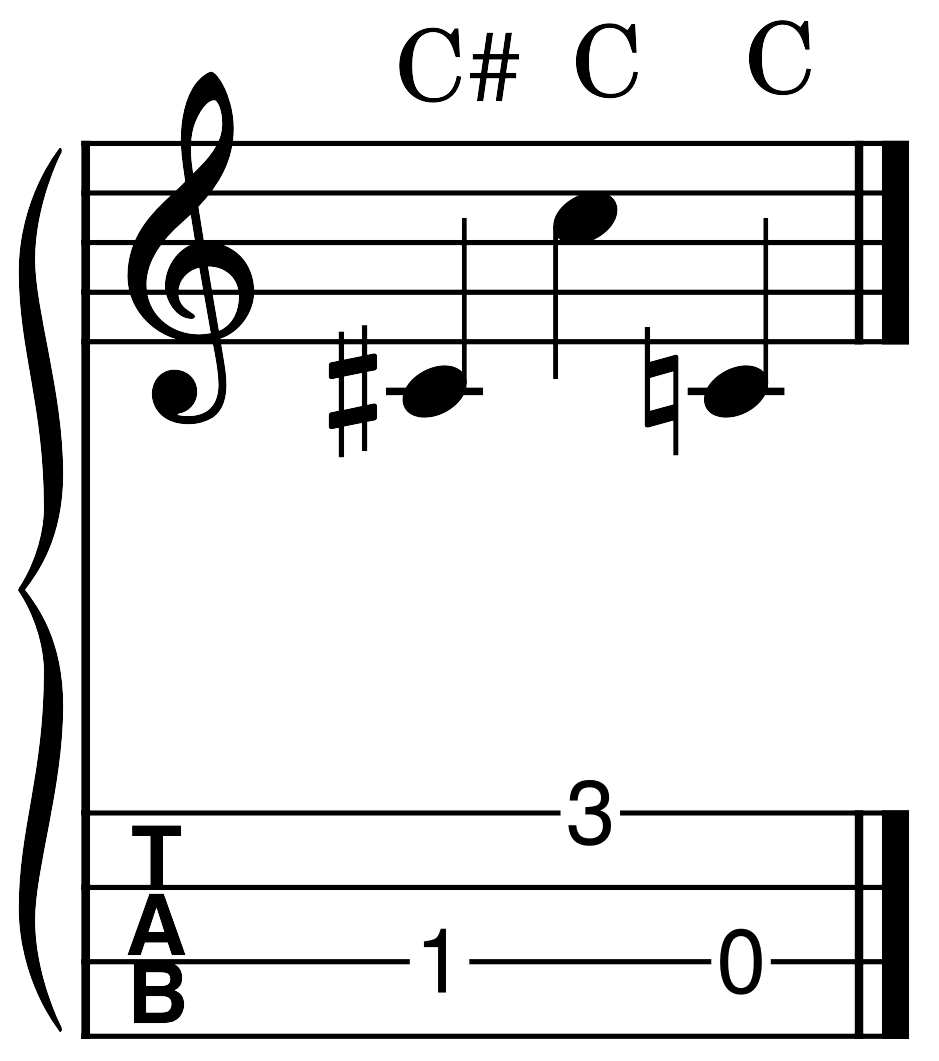
\includegraphics[height=0.15\textheight]{../../MuseScore/Ukulele/UkuleleSharpApplyExample.png}
		\caption{Usage of sharps and naturals}
		\label{fig:ukulele_usage_of_sharps_and_naturals}
	\end{subfigure}
	\hfill
	\begin{subfigure}[b]{0.45\textwidth}
		\centering
		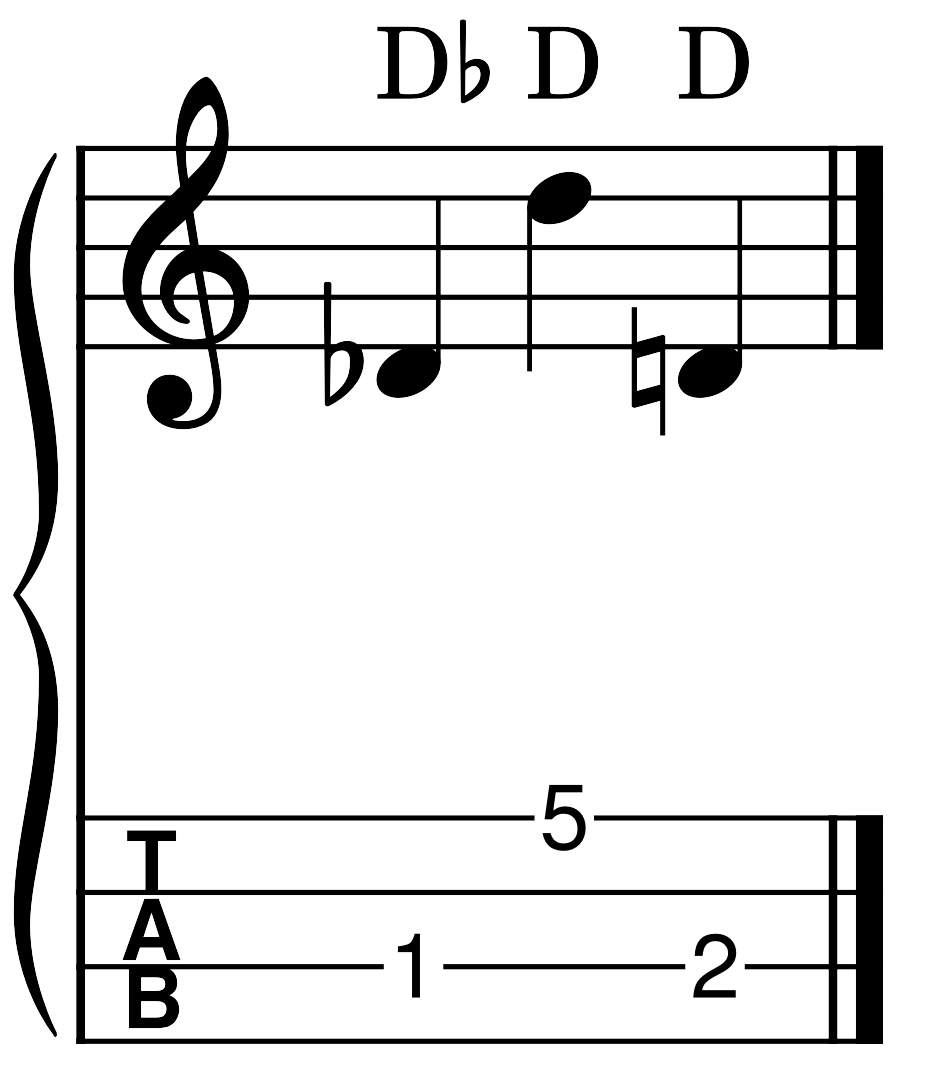
\includegraphics[height=0.15\textheight]{../../MuseScore/Ukulele/UkuleleFlatApplyExample.png}
		\caption{Usage of flats and naturals}
		\label{fig:ukulele_usage_of_flats_and_naturals}
	\end{subfigure}
	\caption{Sharps, flats and naturals}
\end{figure}

Sometimes a song uses a note with a flat or sharp a lot of times. It can then be considered to be in a certain key (we will come back to that later). It is then not desired to add sharps/flats all over the sheet music. That could get messy. Instead, the sharps/flats used for the song are shown at the beginning of the piece and apply to all pitches of the notes (unless natural symbols are used). Note that this is different compared to adding sharps inside a measure, there it is only applied to that specific pitch.

See for example \autoref{fig:ukulele_sharps_at_start_of_music} and \autoref{fig:ukulele_flats_at_start_of_music}.

\begin{figure}[h]
	\centering
	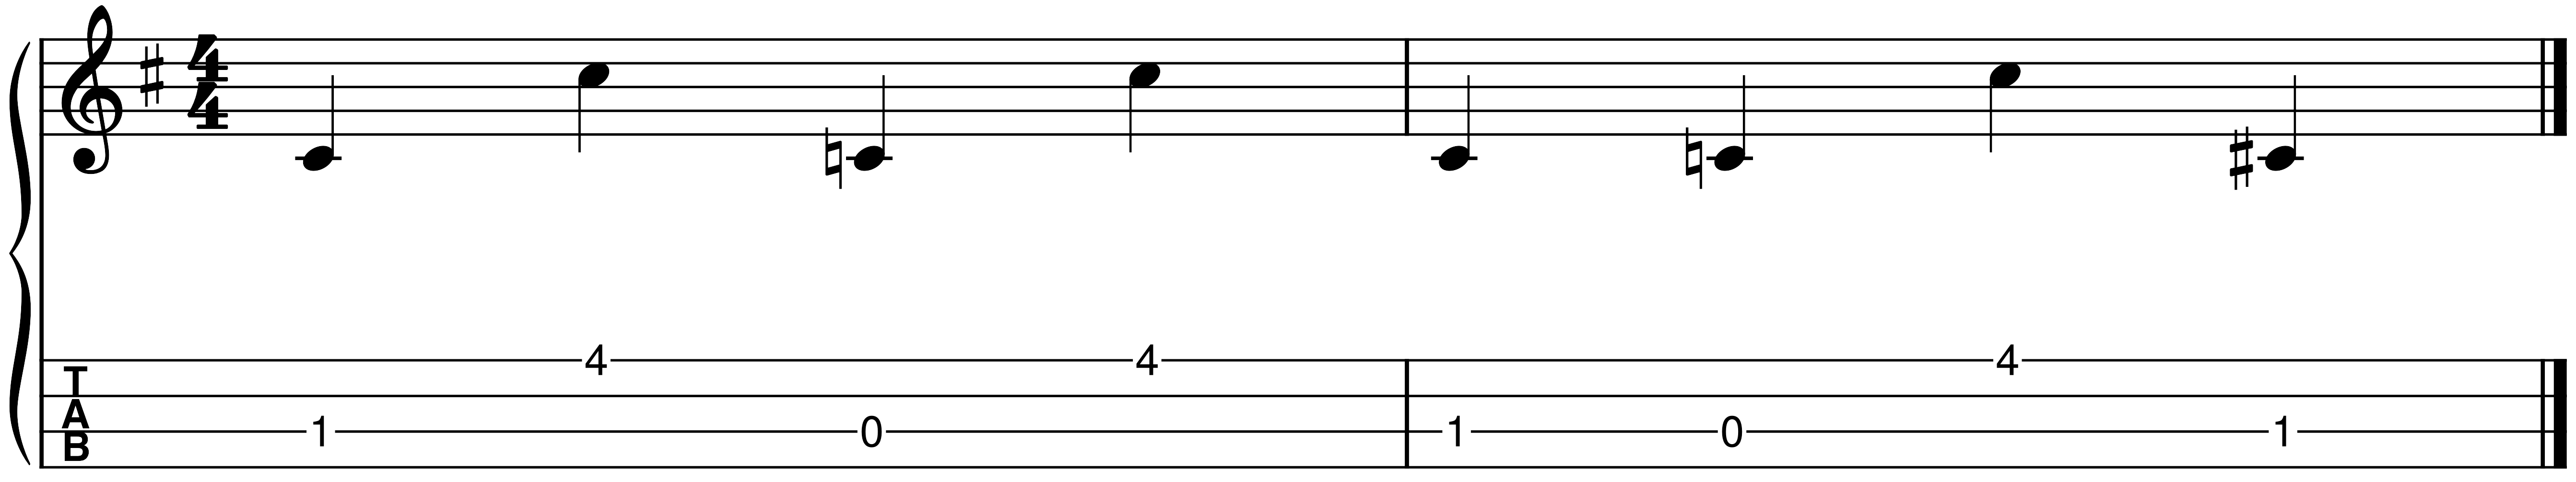
\includegraphics[width=\textwidth]{../../MuseScore/Ukulele/UkuleleKeySharpExample.png}
	\caption{Example of adding sharps at the beginning of the music}
	\label{fig:ukulele_sharps_at_start_of_music}
\end{figure}

\begin{figure}[h]
	\centering
	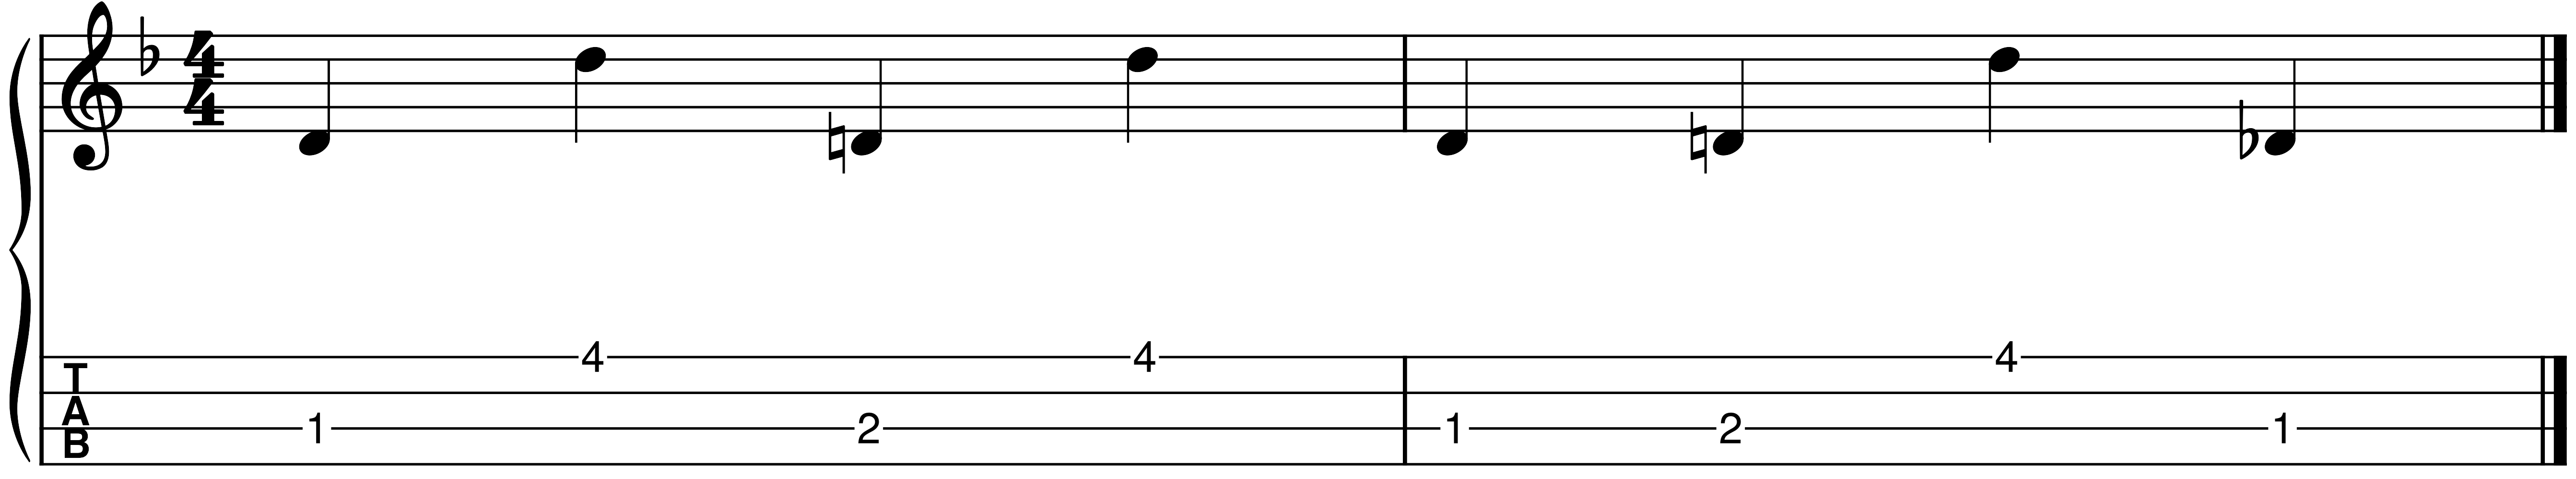
\includegraphics[width=\textwidth]{../../MuseScore/Ukulele/UkuleleKeyFlatExample.png}
	\caption{Example of adding flats at the beginning of the music}
	\label{fig:ukulele_flats_at_start_of_music}
\end{figure}

\newpage

Before playing some pieces to learn the sharps and flats, lets first show the sharps and flats on the fretboard again:

\begin{figure}[h]
	\centering
	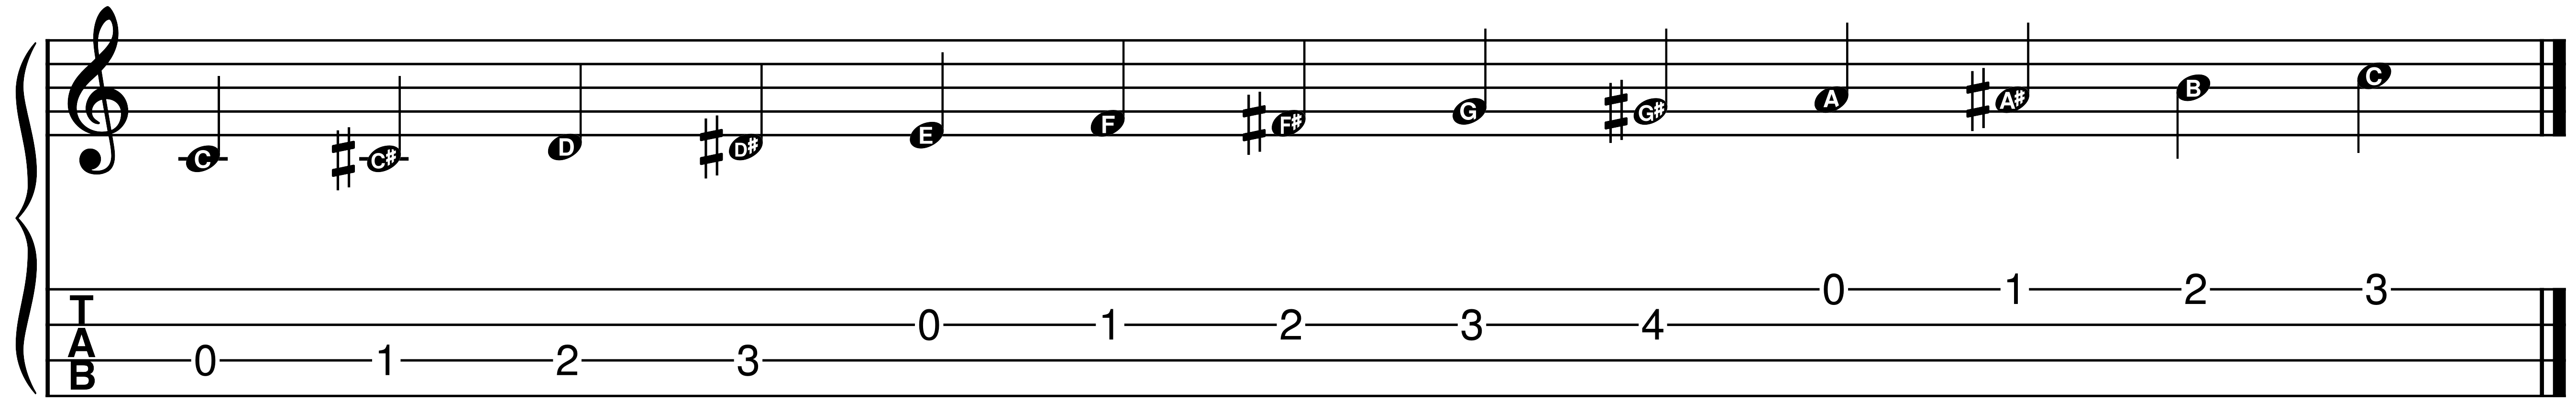
\includegraphics[width=\textwidth]{../../MuseScore/Ukulele/UkuleleChromaticNotesSharpsMultiString.png}
	\caption{An octave from C to C on strings 1 to 3 with sharps}
	\label{fig:ukulele_multi_string_octave_sharps_chapter_music_notation}
\end{figure}

\begin{figure}[h]
	\centering
	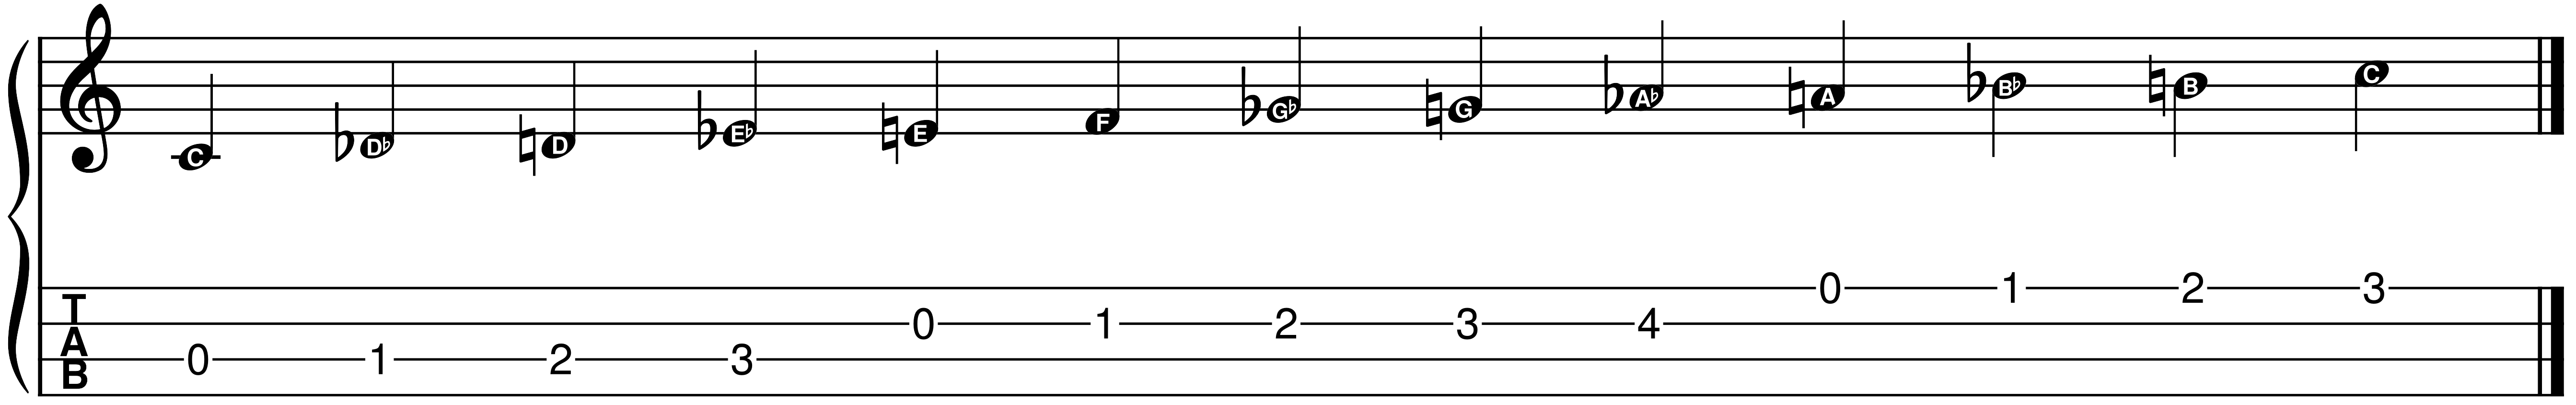
\includegraphics[width=\textwidth]{../../MuseScore/Ukulele/UkuleleChromaticNotesFlatsMultiString.png}
	\caption{An octave from C to C on strings 1 to 3 with flats and naturals}
	\label{fig:ukulele_multi_string_octave_flats_chapter_music_notation}
\end{figure}

Also remember that between each note, except for B-C and E-F, there are two half steps. Between B-C and E-F there is only one half step.

\begin{table}[h]
	\centering
	\begin{tabular}{*{12}{P{5mm}}}
		\large{A} & \large{A\sharp} & \large{B} & \large{C} & \large{C\sharp} & \large{D} & \large{D\sharp} & \large{E} & \large{F} & \large{F\sharp} & \large{G} & \large{G\sharp} \\ \\
		\large{A} & \large{B\flat} & \large{B} & \large{C} & \large{D\flat} & \large{D} & \large{E\flat} & \large{E} & \large{F} & \large{G$\flat$}& \large{G} & \large{A\flat}
	\end{tabular}
	\caption{Sharp and flat intervals}
	\label{tab:ukulele_sharp_flat_intervals_chap_4}
\end{table}

Remember that a sharp and flat simply move the note a half step up or down respectively. So what would happen when the E note gets a $\sharp$? It would become an F. And what does an F$\flat$ resolve to? An E indeed. The same holds for the B-C interval. B$\sharp$ is the same as a C and a C$\flat$ is the same as a B.

\newpage

The music shown in \autoref{fig:ukulele_memory_cats} doesn't show any symbols in the notes. But it does show two flat symbols at the beginning of the music. In this case it shows a B\flat and an E\flat. Note that these apply to any pitch of the B and E notes in the music.

An empty tablature staff has been added. You can fill this in yourself to help learn the position of the (flat) notes on the fretboard.

\begin{figure}[h]
	\centering
	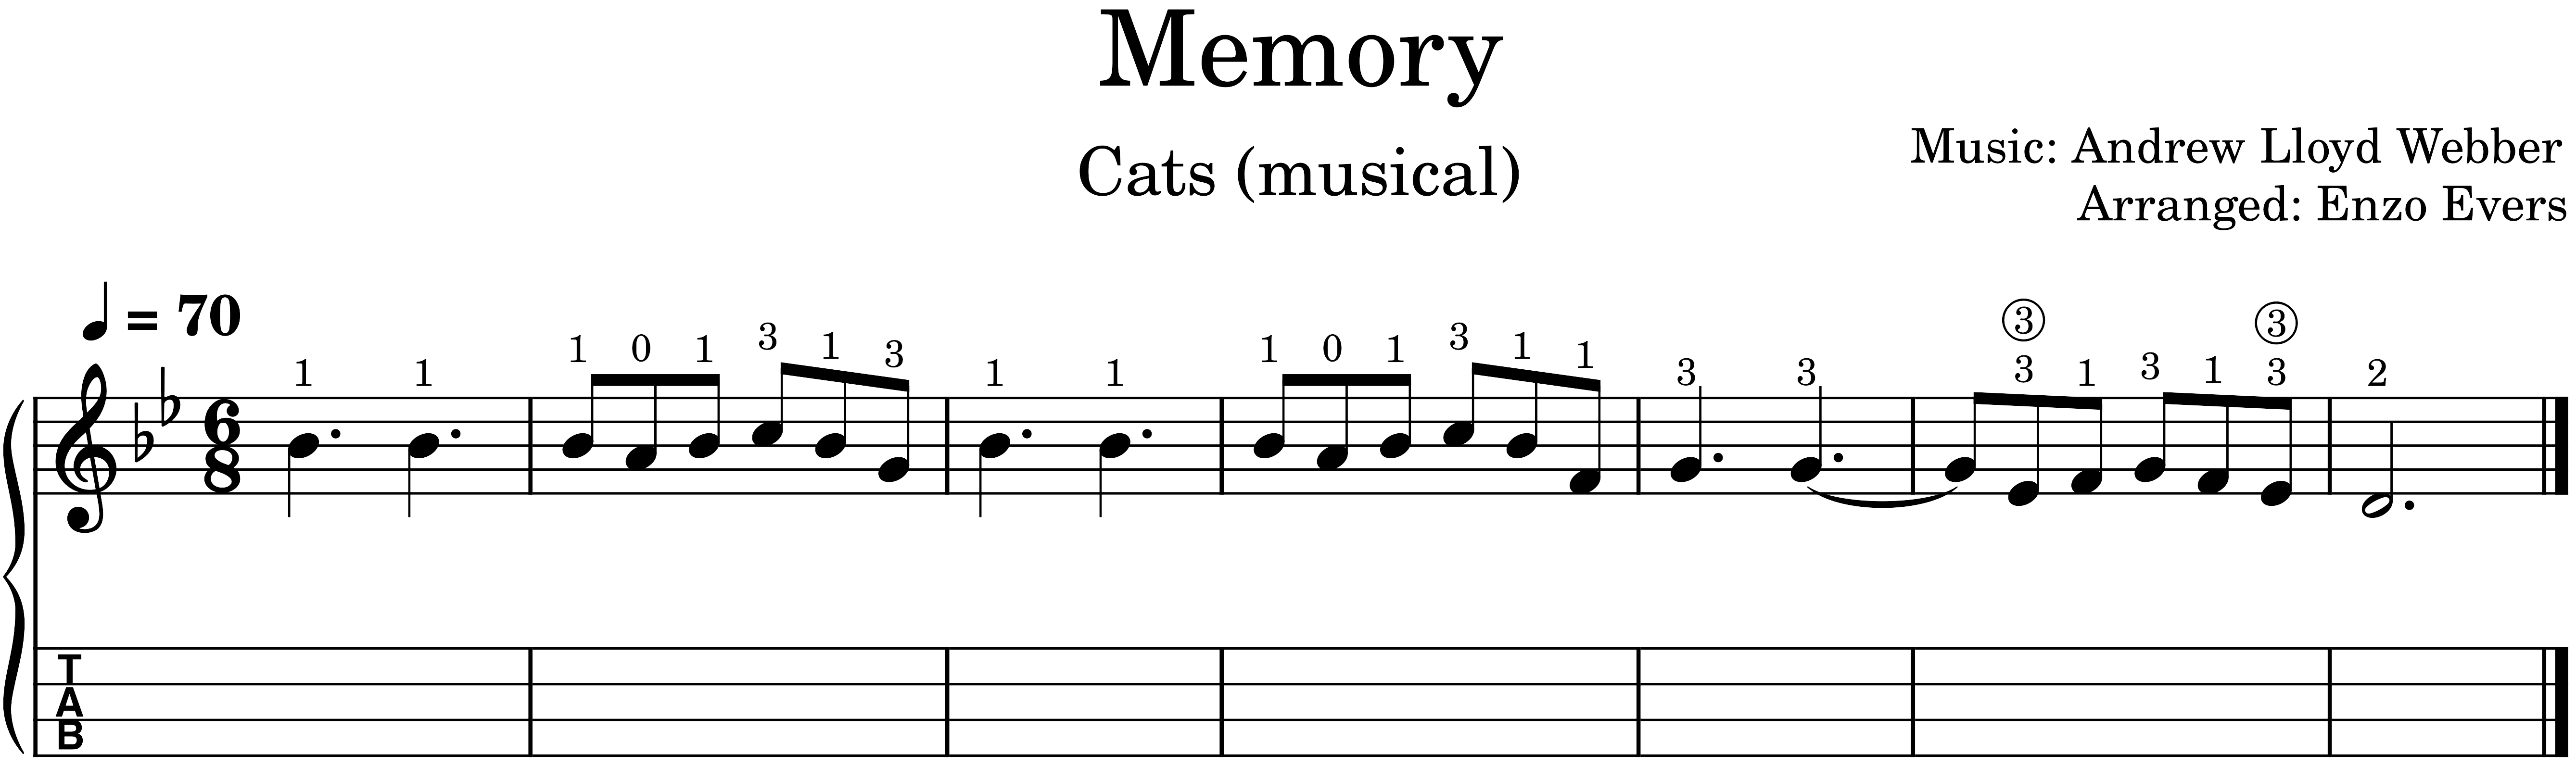
\includegraphics[width=\textwidth]{../../MuseScore/Ukulele/UkuleleMemoryCats.png}
	\caption{Memory from the Cats musical}
	\label{fig:ukulele_memory_cats}
\end{figure}

Happy birthday uses a music-wide F\sharp. It also introduces one new note. The high D note (in measure 6). This note has not been played in earlier songs yet. But try to see if you can figure out the position based on your knowledge of the note intervals (\autoref{tab:ukulele_sharp_flat_intervals_chap_4}) and how that relates to the frets on the fretboard. If you want to know the answer, have a look at \autoref{fig:ukulele_usage_of_flats_and_naturals}.

\begin{figure}[h]
	\centering
	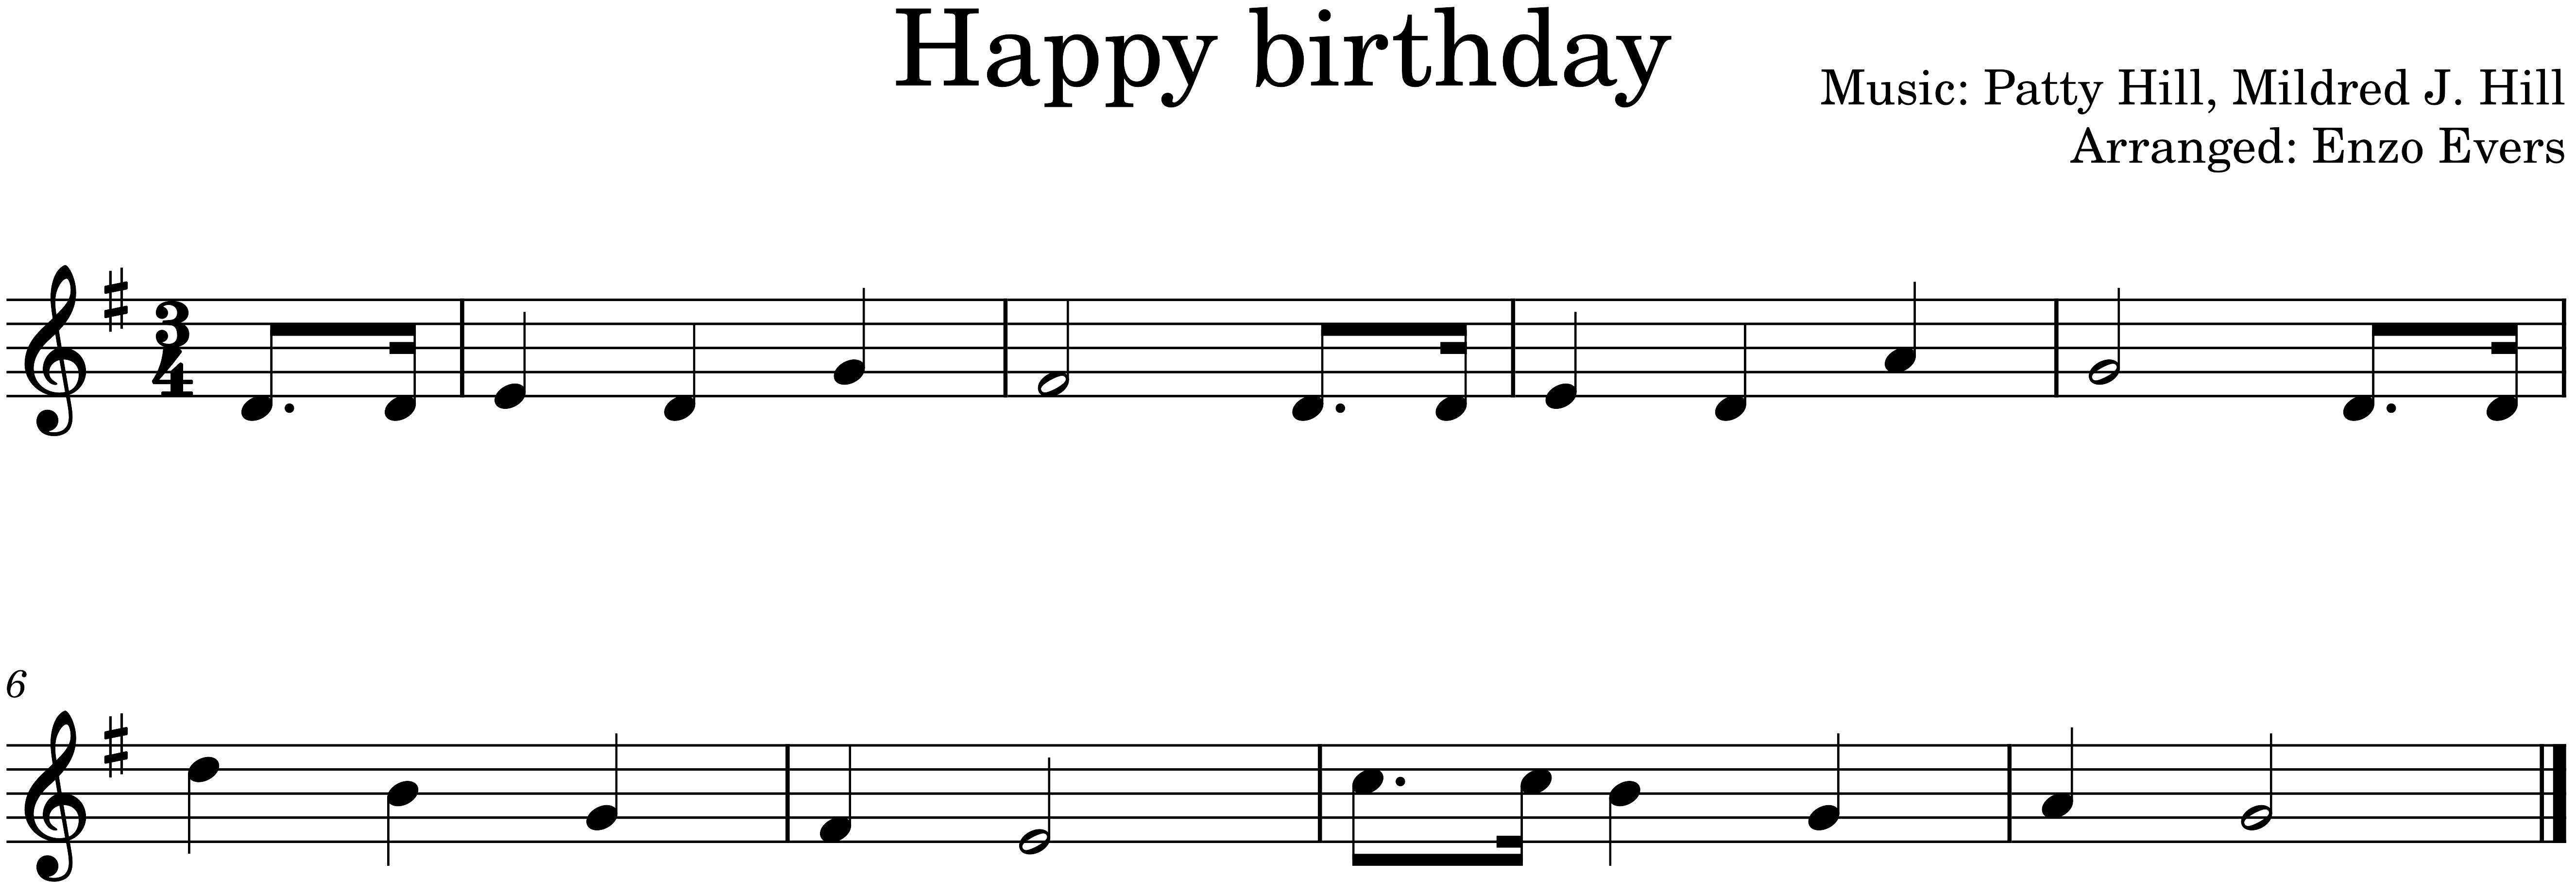
\includegraphics[width=\textwidth]{../../MuseScore/Ukulele/UkuleleHappyBirthday.png}
	\caption{Happy birthday}
	\label{fig:ukulele_happy_birthday}
\end{figure}

In Hedwig's Theme (see the next page) you will see the usage of sharps, flats, naturals and music-wide sharps. It uses the same music-wide F$\sharp$ as Happy birthday.

To better help learn the position of these notes there is an empty tablature staff added. You can fill this staff with the correct tabs to help you learn.

After that there is the song "He's a pirate" from the "Pirates of the Caribbean" movies. This song doesn't introduce any new notes and is here purely for review.

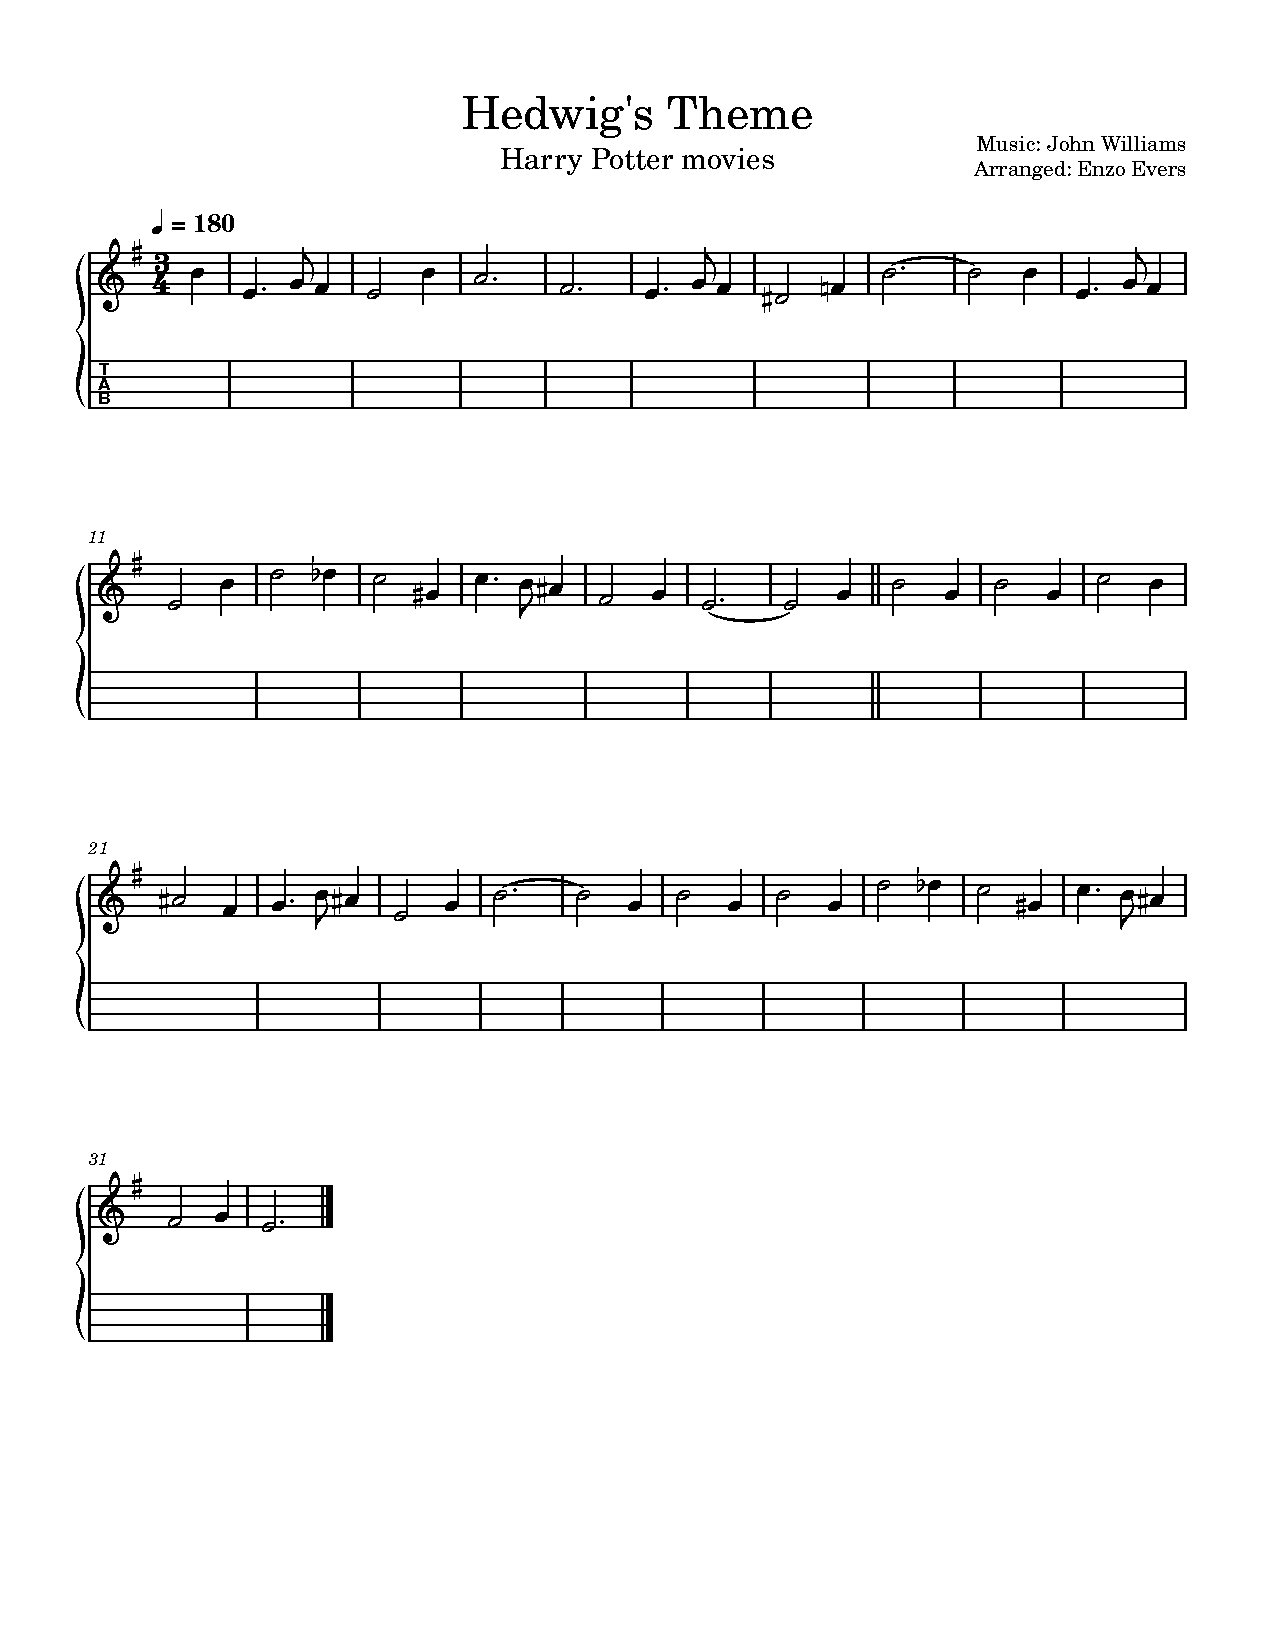
\includepdf[pages=-,pagecommand={\thispagestyle{headings}}]{../../MuseScore/Ukulele/UkuleleHarrysPotterHedwigsTheme.pdf}

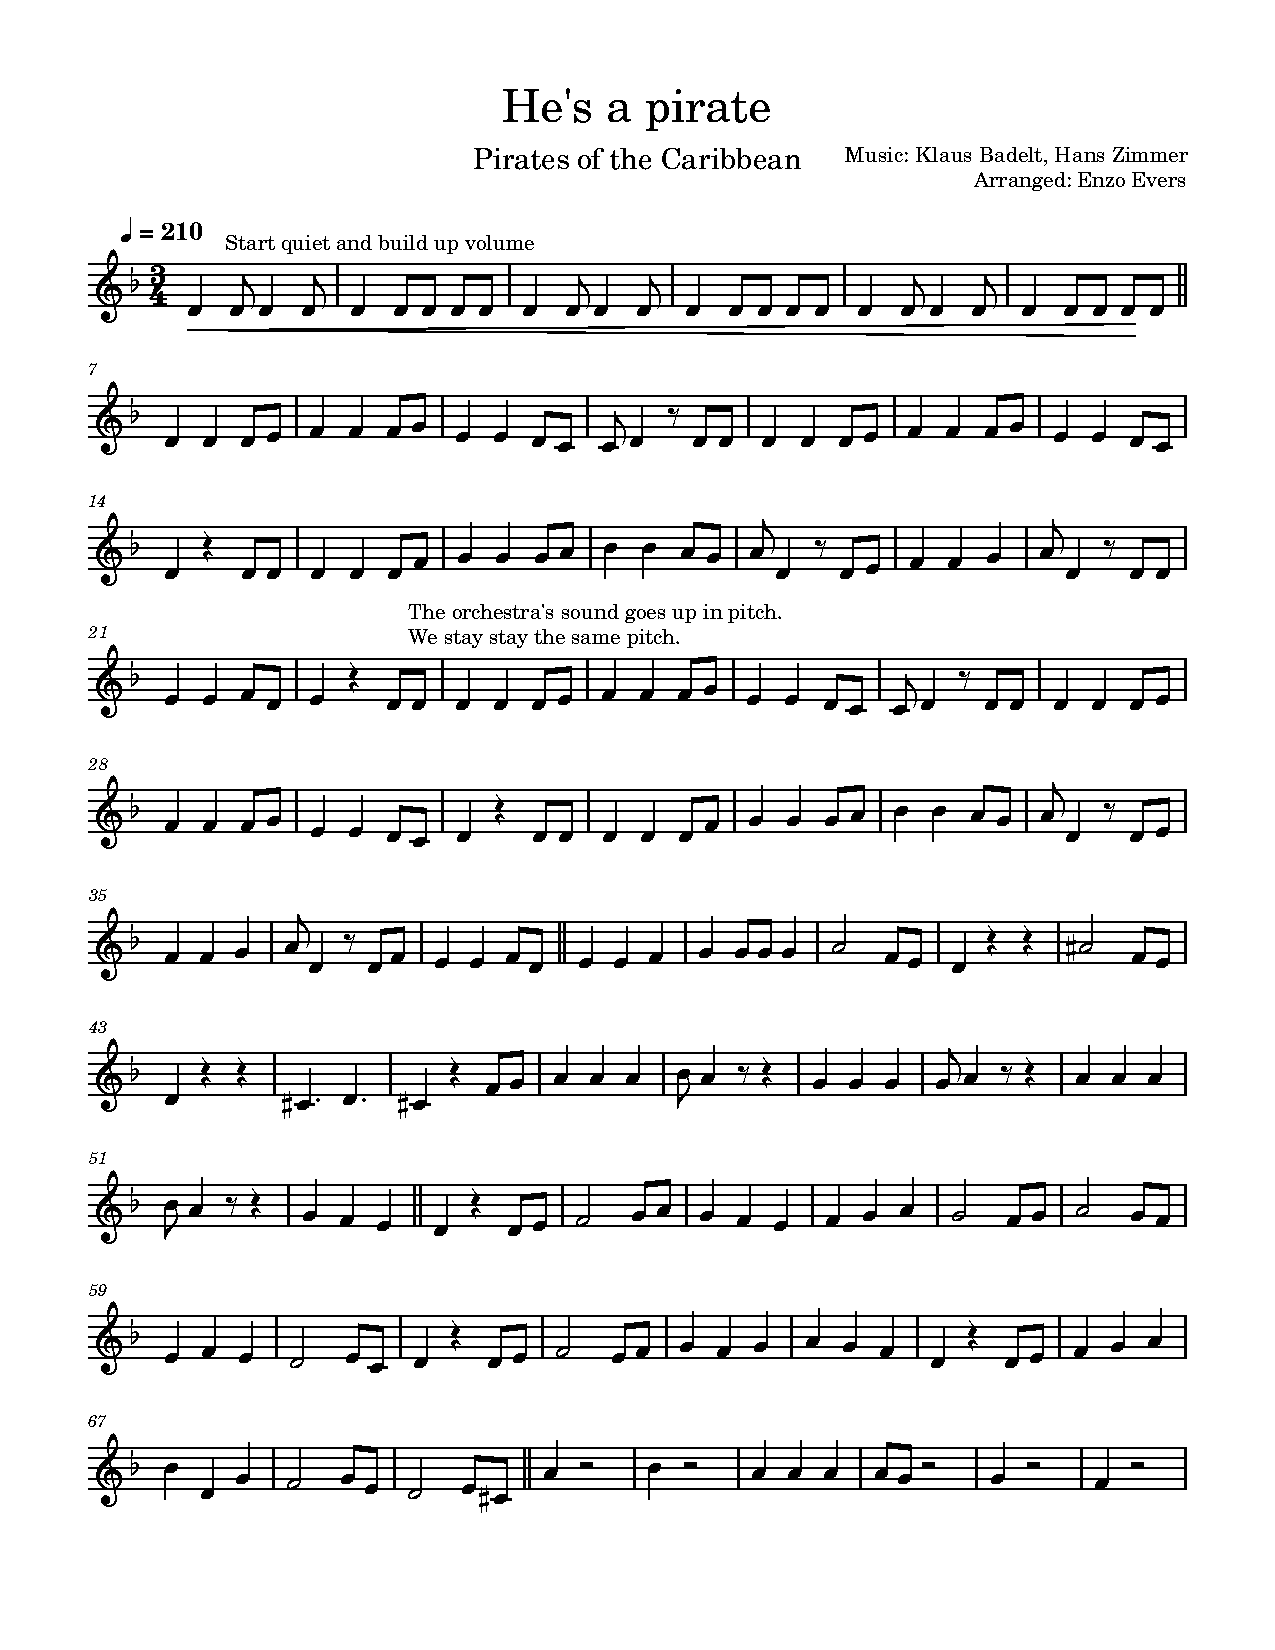
\includepdf[pages=-,pagecommand={\thispagestyle{headings}}]{../../MuseScore/Ukulele/UkuleleHesAPirate.pdf}

The following song introduces two new high notes. The high E and F (see \ref{fig:ukulele_high_e_f_notes}). Note that in \autoref{fig:ukulele_cest_la_vie_chefspecial} all F notes become an F$\sharp$ due to the sharps at the start of the song.

\begin{figure}[h]
	\centering
	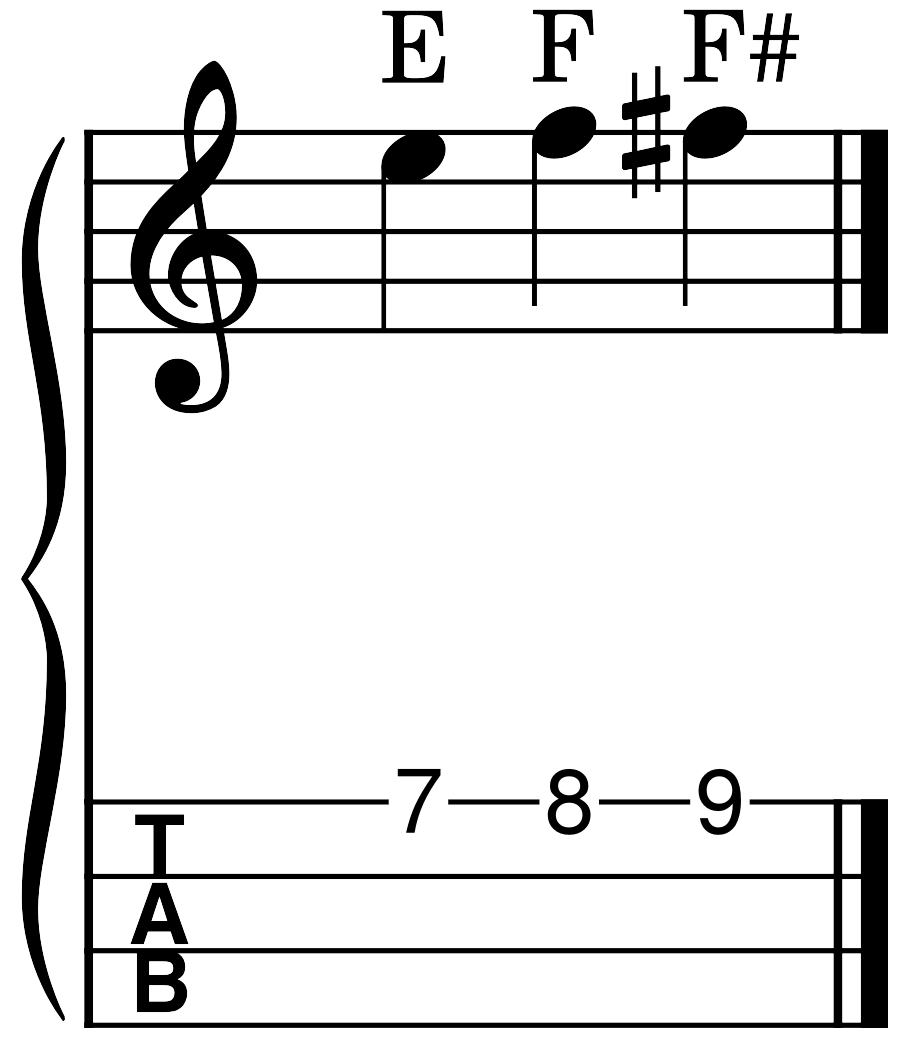
\includegraphics[height=0.12\textheight]{../../MuseScore/Ukulele/UkuleleHighEF.png}
	\caption{Position of the high E, F, and F\sharp notes}
	\label{fig:ukulele_high_e_f_notes}
\end{figure}

The notes here play the singing/melody line. Therefore the chords are placed above the notes to make it easier for two people two play together. One plays the chords, the other the melody. But don't worry about the chords yet. We come to that in the next chapter. The complete song will be learned later on in the book.

Just like with the other songs. Feel free to fill in the tabs to help you learn the notes.

\begin{figure}[h]
	\centering
	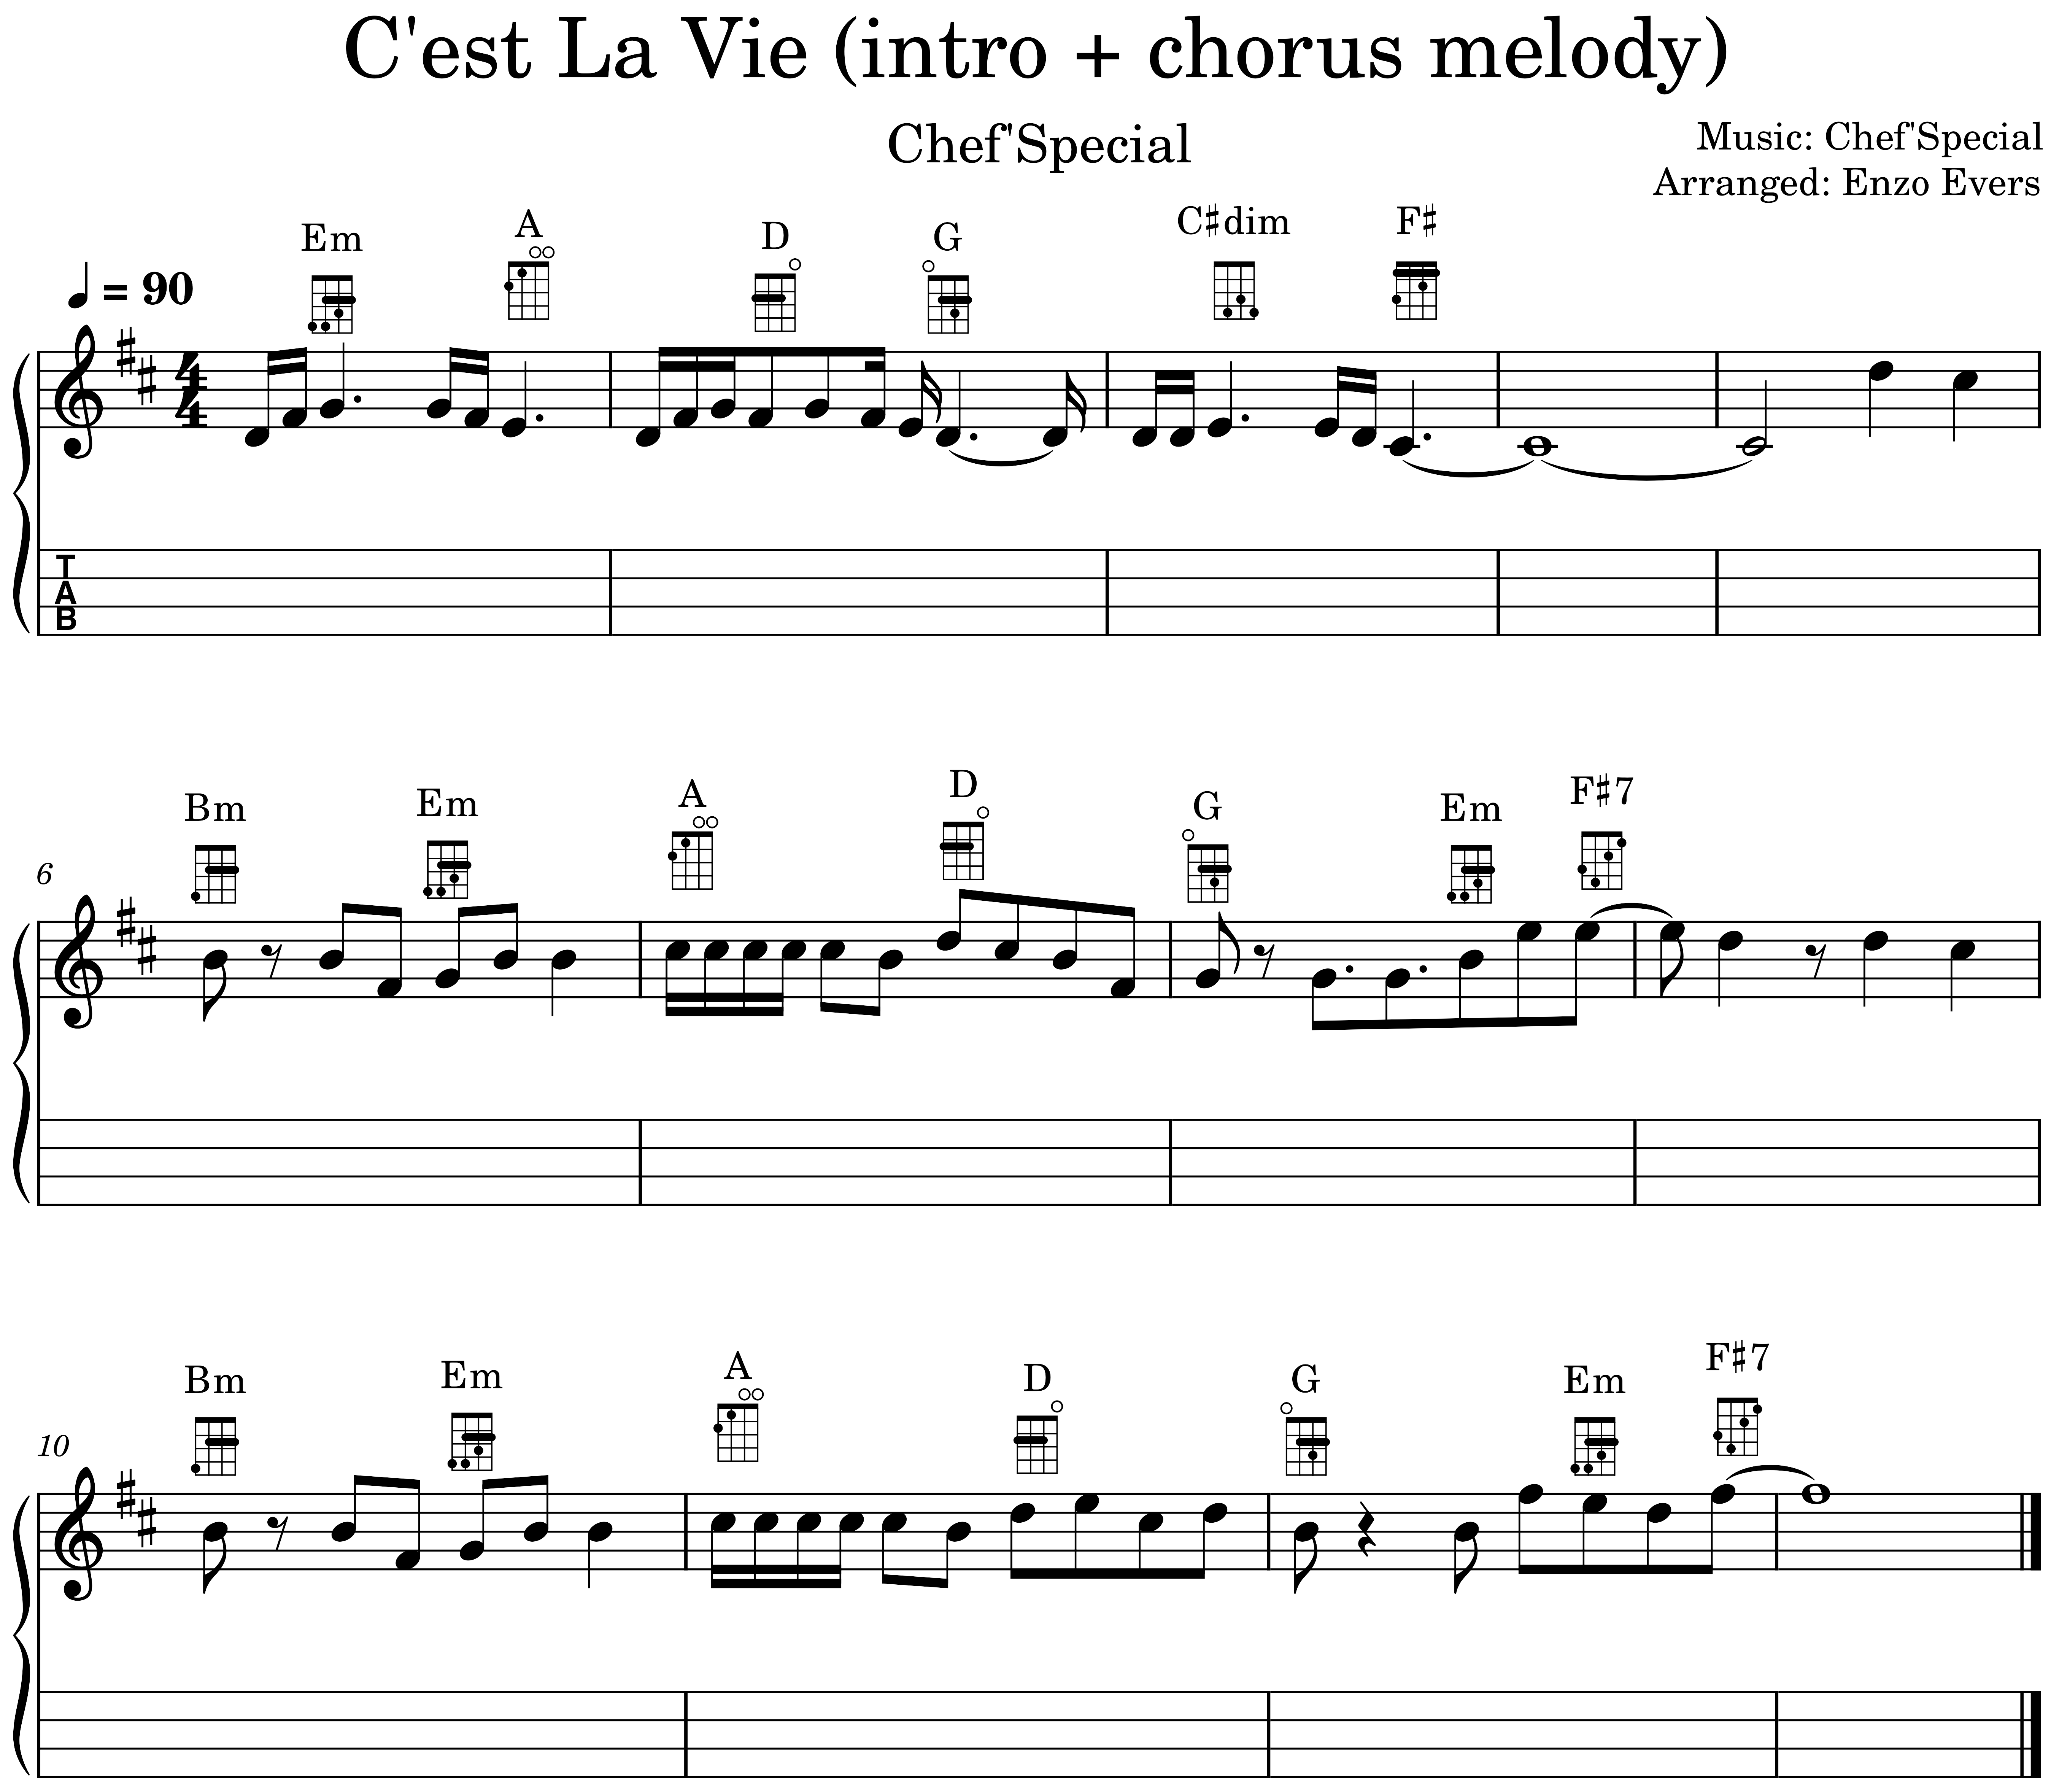
\includegraphics[width=\textwidth]{../../MuseScore/Ukulele/UkuleleCestLaVieChefSpecial_IntroChorus.png}
	\caption{C'est La Vie - Chef'Special}
	\label{fig:ukulele_cest_la_vie_chefspecial}
\end{figure}
